\section{Introduction}

Efficient computation of certain matrix functions is one of the core topics in numerical linear
algebra. Among other applications (see Chapter 2 of \cite{higham2008functions} for a
comprehensive list of the applications), matrix functions often arise in solutions of
differential equations:
\begin{itemize}
    \item The exact solution to the initial value problem
        \begin{equation*}
            \dot{\mathbf{x}}(t) = A \mathbf{x}(t),\;
            \mathbf{x}(0) = \mathbf{x_0}, \quad
            \mathbf{x} \in \mathbb{C}^{n},
            A \in \mathbb{C}^{n \times n}
        \end{equation*}
        is given by $\mathbf{x}(t) = e^{tA} \mathbf{x_0}$.
        More generally, with some assumptions on the smoothness
        of a non-linear function $g$, the solution to the problem
        \begin{equation}
            \label{eq:exponentialintegratorproblem}
            \dot{\mathbf{x}}(t) = A \mathbf{x}(t) + \mathbf{g}(t, \mathbf{x}(t)), \; \mathbf{x}(0) = \mathbf{x_0},
            \quad \mathbf{x} \in \mathbb{C}^{n}, A \in \mathbb{C}^{n \times n}
        \end{equation}
        is given by
        \begin{equation}
            \label{eq:exponentialintegratorsolution}
            \mathbf{x}(t) = e^{tA} \mathbf{x_0} + \int_{0}^{t}{e^{(t-s)A} \mathbf{g}(t, x(s)) ds}.
        \end{equation}

    \item The exact solution to the initial value problem
    \begin{equation*}
        \dot{X}(t) = A X(t) + X(t) B, \; X(0) = C, \quad X \in \mathbb{C}^{m \times n}, A \in \mathbb{C}^{m \times m}, B \in \mathbb{C}^{n \times n}
    \end{equation*}
    is given by $X(t) = e^{tA} C e^{tB}$.

    \item The second order differential initial value problem
    \begin{equation*}
        \ddot{X}(t) + A X(t) = 0, \; X(0) = B, \dot{X}(0) = C, \quad A, X \in \mathbb{C}^{n \times n}
    \end{equation*}
    has the solution
    \begin{equation*}
        X(t) = \cos(t \sqrt{A}) B + (\sqrt{A})^{-1} \sin(t \sqrt{A}) C
        = \cos(t \sqrt{A}) B + t \mathrm{sinc}(t \sqrt{A}) C,
    \end{equation*}
    where the scalar sinc function is defined by $\mathrm{sinc}(z) = \sin(z) / z$.
\end{itemize}

Other notable applications of matrix functions include the differential equations
appearing in nuclear magnetic resonance, Markov models, and control theory.

Nonlinear ordinary differential equations of type \eqref{eq:exponentialintegratorproblem}
usually arise in spatial discretization of time dependant partial differential equations.
Exponential integrators are a class of numerical methods for solving these problems, especially
when they are stiff. These methods treat the linear term of \eqref{eq:exponentialintegratorsolution}
exactly and integrate the other term numerically. They are based on the premise that most of the
stiffness of the problem originates from the matrix $A$, and not from the non-linear part. The matrix
$A$ that appears in such problems is typically large and sparse. In several applications, this matrix
is symmetric and semi-definite positive, which is the case we consider in this work.
A presentation and review of these methods is given in \cite{minchev2005review}.
A core step in these methods is the efficient computation of matrix-vector multiplications where
the matrix is $\exp(tA)$ or $\varphi_p(tA)$ (to be defined later) for a suitable parameter $t$.

In this work, we focus on the computation of the action of matrix exponentials and
$\varphi$-functions on given vectors using Krylov subspace methods.
In \autoref{sec:matrixfunctions}, basic definitions and properties of the matrix functions
regarded in this work are given. In \autoref{sec:methods}, we present the theoretical ideas
and the numerical methods. The definitions of polynomial and rational Krylov subspaces,
the Arnoldi algorithm, the approximation methods, and the reference methods are presented.
Furtheremore, theoretical bounds for the error of the polynomial Krylov subspace approximation
are derived in this section. In \autoref{sec:experiments}, we present the details of our
implementations of the methods in \autoref{sec:methods} and the results of numerical experiments.
In \autoref{sec:resultstrigonometricfunctions}, computing the action of three trigonometric
matrix functions on certain vectors is motivated and the methods are applied and evaluated on them.

\section{Matrix Functions}
\label{sec:matrixfunctions}

\subsection{Definitions}
This section reviews the basic definition and properties of matrix functions
discussed in detail in \cite{higham2008functions}.
Let $A \in \mathbb{C}^{n \times n}$ have $s$ distinct eigenvalues $\sigma(A) = \{\lambda_k\}_{k=1}^{s}$.
$A$ can be expressed in the Jordan canonical form as $A = ZJZ^{-1} = Z \diag(J_k)_{k=1}^{s}
Z^{-1}$. Let $m_k$ denote the size of the largest Jordan block associated
with $\lambda_k$. The matrix function associated with a scalar function $f$
is defined by $f(A) := g(A)$, where $g(z)$ is the unique Hermite interpolating
polynomial of degree less than $\sum_{k=1}^{s}{m_k}$, which satisfies
\begin{equation}
    \frac{\partial^j}{\partial z^j}g(\lambda_k) = \frac{\partial^j}{\partial z^j}f(\lambda_k),
    \quad \forall j \in \{0, 1, \dots, m_k-1\},
    \quad \forall k \in \{1, 2, \dots, s\},
\end{equation}
assuming that all required derivatives of $f(z)$ exist.

Equivalently, $f(A)$ can also be defined as $f(A) := Z \diag(f(J_k))_{k=1}^{s} Z^{-1}$ where
\begin{equation*}
    f(J_k) =
    \begin{bmatrix}
    f(\lambda_k) & f'(\lambda_k)  & \frac{1}{2} f^{(2)}(\lambda_k) & \cdots & \frac{f^{(m_k-1)}(\lambda_k)}{(m_k - 1)!}\\
    & f(\lambda_k) & f'(\lambda_k) & \cdots & \frac{f^{(m_k-2)}(\lambda_k)}{(m_k - 2)!} \\
    &  & f(\lambda_k) & \ddots & \vdots \\
    &  &  & \ddots & f'(\lambda_k)\\
    &  &  &  & f(\lambda_k)
    \end{bmatrix}.
\end{equation*}

If $A = Z \diag(\lambda_k)_{k=1}^{n} Z^{-1}$ is diagonalizable, we have
\begin{equation}
    \label{eq:matrixfunctiondiagonal}
    f(A) = Z \diag(f(\lambda_k))_{k=1}^{n} Z^{-1}.
\end{equation}

A third equivalent definition is via the Cauchy's integral formula and it reads
\begin{equation}
    f(A) := \frac{1}{2 \pi i} \int_{\Gamma}{f(z)(zI - A)^{-1} dz},
\end{equation}
assuming that $f$ is analytic on and inside a closed contour $\Gamma$ that encloses $\sigma(A)$.

\subsection{Matrix Exponential}
The matrix function attributed to the scalar exponential function is called
matrix exponential and is defined~\cite{higham2008functions} as
\begin{equation}
    \label{eq:matrixexponentialdefinition}
    \exp(A) = \sum_{k=0}^{\infty}{\frac{1}{k!} A^k}.
\end{equation}

Some properties of the matrix exponential follows:
\begin{itemize}
    \item By taking the conjugate transpose of \eqref{eq:matrixexponentialdefinition},
        it can be concluded that $\exp(A^{*}) = \exp(A)^{*}$.
    \item For all $A, B \in \mathbb{C}^{n \times n}$ that satisfy $AB = BA$,
        we have $\exp(A + B) = \exp(A) \exp(B)$.
    \item $\exp(A)$ is always invertible and its inverse is $\exp(A)^{-1} = \exp(-A)$.
    \item The derivative of $\exp(tA)$ with respect to a scalar $t$ is given by
        $\frac{\mathrm{d}}{\mathrm{d} t} (\exp(tA)) = A \exp(tA)$.
    \item The determinant of $\exp(A)$ is the exponential of the trace of
        $A$: $\det(\exp(A)) = \exp(\trace(A))$.
\end{itemize}

\subsection{\texorpdfstring{$\varphi$}{Phi}-Fxunctions}
In the core of exponential integrators for solving stiff problems of type
\eqref{eq:exponentialintegratorproblem}, lies the computation of the application of
$\varphi$-functions on vectors from the previous iterations. Accurate and efficient computation of
these vectors is vital for implementation of exponential integrators.
For a scalar argument $z \in \mathbb{C}$, the $\varphi$-functions are
defined~\cite{higham2008functions} as
\begin{equation}
    \label{eq:scalarphifunctionsdefinition}
    \begin{aligned}
        & \varphi_0(z) = e^z,\\
        & \varphi_p(z) = \frac{1}{(p-1)!} \int_{0}^{1}{e^{(1 - \theta)z} \theta^{p-1} d\theta},
        \quad p \in \mathbb{N^*}.
    \end{aligned}
\end{equation}
The parameter $p$ is related to the order of the exponential integrator and it typically takes
values less than $5$.
The $\varphi$-functions satisfy~\cite{higham2008functions} the recurrence relation
\begin{equation}
    \label{eq:scalarphifunctionsrecurrence}
    \begin{aligned}
        & \varphi_p(z) = z^{-1} \left[ \varphi_{p-1}(z) - \frac{1}{(p-1)!} \right] ,
        & z \neq 0,
        \\
        & \varphi_p(z) = \frac{1}{p!},
        & z = 0,
    \end{aligned}
\end{equation}
for all $p \in \mathbb{N^*}$.

The evaluation of the first three scalar $\varphi$-functions on the left half complex plane
is illustrated in \autoref{fig:scalarphifunctionscomplexplane}. Note that the gradients are
smaller for higher $p$'s.

We can use \eqref{eq:scalarphifunctionsrecurrence} recursively as
\begin{equation*}
    \begin{aligned}
        \varphi_p(z) & = z^{-1} \varphi_{p-1}(z) - \frac{1}{(p-1)!} z^{-1} \\
        & = z^{-1} \left[ z^{-1} \varphi_{p-2}(z) - \frac{1}{(p-2)!} z^{-1} \right] - \frac{1}{(p-1)!} z^{-1} \\
        & = z^{-2} \varphi_{p-2}(z) - \frac{1}{(p-2)!} z^{-2} - \frac{1}{(p-1)!} z^{-1} \\
        & = \cdots \\
        & = z^{-p} \varphi_{0}(z) - \frac{1}{0!} z^{-p} - \frac{1}{1!} z^{-(p-1)} - \frac{1}{2!} z^{-(p-2)} - \cdots - \frac{1}{(p-1)!} z^{-1} \\
        & = z^{-p} \exp(z) - \sum_{k=0}^{p-1}{\frac{1}{k!}z^{-(p-k)}}
        \end{aligned}
\end{equation*}
to derive a closed form for $\varphi_p$:
\begin{equation}
    \label{eq:scalarphifunctionsclosedform}
    \varphi_p(z) = z^{-p} \left( \exp(z) - \sum_{k=0}^{p-1}{\frac{1}{k!}z^{k}} \right), \quad z \neq 0.
\end{equation}

For an invertible matrix $A \in \mathbb{C}^{n \times n}$, we can do the same steps
and use \eqref{eq:matrixexponentialdefinition} to get
\begin{equation}
    \label{eq:matrixphifunctionsclosedform}
    \varphi_p(A) = A^{-p} \left( \exp(A) - \sum_{k=0}^{p-1}{\frac{1}{k!}A^{k}} \right)
    = \sum_{k=p}^{\infty}{\frac{1}{k!} A^{k-p}}.
\end{equation}

\begin{remark}
    Using \eqref{eq:scalarphifunctionsclosedform} and \eqref{eq:matrixphifunctionsclosedform}
    for computing the $\varphi$-functions suffers from catastrophic cancellation and
    is numerically unstable. These relations are only used in the theoretical proofs.
\end{remark}

\begin{figure}[h]
    \centering
    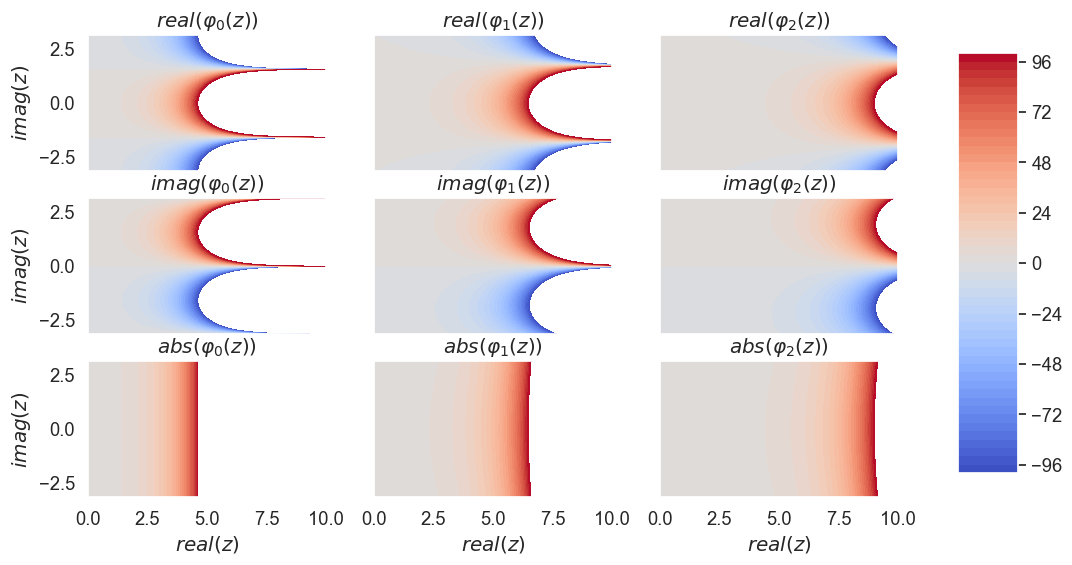
\includegraphics[width=.7\textwidth]{img/scalarcomplexplane.png}
    \caption{
        Evaluation of scalar $\varphi$-functions on the complex plane.
        The values that are out of the range of the color bar are not
        visualized (white areas).
        }
    \label{fig:scalarphifunctionscomplexplane}
\end{figure}

\subsection{Trigonometric Matrix Functions}
\label{sec:trigonometricmatrixfunctions}

The two most important trigonometric functions, sine and cosine, are defined
\cite{higham2008functions} for all $A \in \mathbb{C}^{n \times n}$ by
\begin{equation}
    \label{eq:matrixcosinedefinition}
    \cos(A) = I - \frac{A^2}{2!} + \frac{A^4}{4!} - \frac{A^6}{6!} + \cdots
    = I + \sum_{k=1}^{\infty}{\frac{(-1)^k}{(2k)!} A^{2k}};
\end{equation}
and
\begin{equation}
    \label{eq:matrixsinedefinition}
    \sin(A) = A - \frac{A^3}{3!} + \frac{A^5}{5!} - \frac{A^7}{7!} + \cdots
    = A + \sum_{k=1}^{\infty}{\frac{(-1)^k}{(2k+1)!} A^{2k+1}}.
\end{equation}
The matrix sinc function associated with the scalar sinc function
$\mathrm{sinc}(z) = \sin(z) / z$ is defined by
\begin{equation}
    \label{eq:matrixsincdefinition}
    \begin{aligned}
        \mathrm{sinc}(A) & = A^{-1} \sin(A)
        = I - \frac{A^2}{3!} + \frac{A^4}{5!} - \frac{A^6}{7!} + \cdots \\
        & = I + \sum_{k=1}^{\infty}{\frac{(-1)^k}{(2k+1)!} A^{2k}}.
    \end{aligned}
\end{equation}
Some properties of the matrix sine and cosine follows:
\begin{itemize}
    \item The matrix analoge of Euler's formula reads $e^{iA} = \cos(A) + i \sin(A)$.
    \item For all $A \in \mathbb{C}^{n \times n}$ we have $\cos(A) = \frac{1}{2} (e^{iA} + e^{-iA})$.
    \item For all $A \in \mathbb{C}^{n \times n}$ we have $\sin(A) = \frac{1}{2i} (e^{iA} - e^{-iA})$.
    \item For all $A \in \mathbb{C}^{n \times n}$ we have $\cos^2(A) + \sin^2(A) = I$.
    \item For real $A \in \mathbb{R}^{n \times n}$ we have $\cos(A) = \mathfrak{Re}(e^{iA})$.
    \item For real $A \in \mathbb{R}^{n \times n}$ we have $\sin(A) = \mathfrak{Im}(e^{iA})$.
\end{itemize}

\section{Methodology}
\label{sec:methods}

\subsection{Krylov Subspaces and the Arnoldi Algorithm}\label{sec:arnoldi}
Given a matrix $A \in \mathbb{C}^{n \times n}$ and a vector $\mathbf{v} \neq 0 \in \mathbb{C}^n$,
the Krylov subspace of dimension $m \leq n$ for them is defined \cite{golub2013matrix} as
\begin{equation}
    \label{eq:krylovsubspacedefinition}
    \begin{aligned}
        \mathcal{K}_m(A, \mathbf{v})
        & :=\setspan\{\mathbf{v}, A\mathbf{v}, A^{2}\mathbf{v}, \dots, A^{m-1}\mathbf{v} \}\\
         & = \{g(A)\mathbf{v} \:|\: g \in \Pi_{m-1} \},
    \end{aligned}
\end{equation}
where $\Pi_{m-1}$ is the set of all polynomials of order less than or equal to $m-1$.
Krylov supspaces are essential in many methods in numerical linear algebra
for solving eigenvalue problems and linear systems.
However, the vectors $\mathbf{v}, A\mathbf{v}, A^{2}\mathbf{v}, \dots, A^{m-1}\mathbf{v}$
are not a good basis for $\mathcal{K}_m(A, \mathbf{v})$. We know from the power method that
these vectors have almost the same direction and converge to the eigenvector paired
with the biggest eigenvalue of $A$.
From the Arnoldi algorithm \cite{trefethen1997numerical} described in Algorithm
\ref{alg:polynomialarnoldi}, we can get an orthonormal basis for $\mathcal{K}_m(A, \mathbf{v})$
and an upper Hessenberg matrix $H_m = V_m^* A V_m$ which is the projection of the action of
$A$ on $\mathcal{K}_m(A, \mathbf{v})$. The Arnoldi factorization reads
\begin{equation}
    \label{eq:arnoldifactorization}
    A V_m = V_m H_m + h_{m+1, m} \mathbf{v_{m+1}} \mathbf{e_m^\top},
\end{equation}
where $\mathbf{e_m}$ is the last canonical basis vector of $\mathbb{R}^{m}$.

\begin{algorithm}[ht!]
    \caption{Standard Arnoldi algorithm}
    \label{alg:polynomialarnoldi}
    \KwIn{
        Matrix $A \in \mathbb{C}^{n \times n}$
        \newline
        Vector $\mathbf{v} \in \mathbb{C}^n \backslash \{0\}$ with $m \le n \in \mathbb{N}$
    }
    \KwOut{Orthonormal basis $V_m = (\mathbf{v_1}, \mathbf{v_2}, \dots, \mathbf{v_m})$ of $\mathcal{K}_m(A, \mathbf{v})$}
    Set $\mathbf{v_1} = \mathbf{v} / \left\| \mathbf{v} \right\|_2$\;
    Set $V_1 = \mathbf{v_1}$\;
    \For{$j = 1, 2, \dots, m$}{
        Compute $\mathbf{w} = A \mathbf{v_j}$\;
        Compute $\mathbf{h_j} = V_j^* \mathbf{w}$\;
        Compute $\mathbf{\tilde{v}_{j+1}} = \mathbf{w} - V_j \mathbf{h_j}$\;
        \If{$\left\| \mathbf{\tilde{v}_{j+1}} \right\|_2 <  0.7 \left\| \mathbf{w} \right\|_2$}{
            Set $\mathbf{\hat{h}_j} = V_j^* \mathbf{\tilde{v}_{j+1}}$\;
            Set $\mathbf{h_j} = \mathbf{h_j} + \mathbf{\hat{h}_j}$\;
            Set $\mathbf{\tilde{v}_{j+1}} = \mathbf{\tilde{v}_{j+1}} - V_j \mathbf{\hat{h}_j}$\;
        }
        Set $h_{j+1, j} = \left\| \mathbf{\tilde{v}_{j+1}} \right\|_2$\;
        Set $\mathbf{v_{j+1}} = \mathbf{\tilde{v}_{j+1}} / h_{j+1, j}$\;
        Set $V_{j+1} = (V_j, \mathbf{v_{j+1}})$\;
    }
\end{algorithm}

Similarly, the rational Krylov subspace \cite{guttel2013rational} associated with
the matrix $A$ and the vector $\mathbf{v}$ with non-zero poles
$\xi_1, \xi_2, \dots, \xi_m \in \overline{\mathbb{C}} := \mathbb{C} \cup \{ \infty\}$
different than all eigenvalues of $A$, is defined as
\begin{equation}
    \label{eq:rationalkrylovsubspacedefinition}
    \begin{aligned}
        \mathcal{Q}_m(A, \mathbf{v})
        & := q_{m-1}(A)^{-1} \setspan\{\mathbf{v}, A\mathbf{v}, A^{2}\mathbf{v}, \dots, A^{m-1}\mathbf{v} \}\\
         & = \{q_{m-1}(A)^{-1} g(A)\mathbf{v} \:|\: g \in \Pi_{m-1} \},
    \end{aligned}
\end{equation}
where $g / q_{m-1}$ is a rational function with a prescribed denominator
\begin{equation*}
    \Pi_{m-1} \ni q_{m-1}(z) = \prod_{j=1}^{m-1}(1 - z / \xi_j).
\end{equation*}

Algorithm \ref{alg:polynomialarnoldi} can be slightly modified to get an orthonormal
basis for $\mathcal{Q}_m(A, \mathbf{v})$. In line 4, instead of $\mathbf{w} = A \mathbf{v_j}$ we set
$\mathbf{w} = (I - A / \xi_j)^{-1} A \mathbf{v_j}$. When the poles are repeated, the algorithm can benefit
a lot from pre-computing the LU decomposition or if applicable the Cholesky factorization
of $(I - A / \xi_j)$ outside of the main loop. These ideas are summerized in Algorithm
\ref{alg:rationalarnoldi}.

\begin{algorithm}[ht!]
    \caption{Rational Arnoldi algorithm with k repeated poles}
    \label{alg:rationalarnoldi}
    \KwIn{
        Matrix $A \in \mathbb{C}^{n \times n}$
        \newline
        Vector $\mathbf{v} \in \mathbb{C}^n \backslash \{0\}$ with $m \le n \in \mathbb{N}$,
        \newline
        Repeated poles $\xi_1, \xi_2, \dots, \xi_k$ with $k \le m$
    }
    \KwOut{Orthonormal basis $V_m = (\mathbf{v_1}, \mathbf{v_2}, \dots, \mathbf{v_m})$ of $\mathcal{K}_m(A, \mathbf{v})$}
    \For{$i = 1, 2, \dots, k$}{
        Compute $P_i L_i U_i = (I - A / \xi_i)$\;
    }
    Set $\mathbf{v_1} = \mathbf{v} / \left\| \mathbf{v} \right\|_2$\;
    Set $V_1 = \mathbf{v_1}$\;
    \For{$j = 1, 2, \dots, m$}{
        Set $i = j - k \left\lfloor \frac{j}{k} \right\rfloor$\;
        Compute $\mathbf{w} = (I - A / \xi_i)^{-1} A \mathbf{v_j}$ using $P_i$, $L_i$, and $U_i$\;
        Compute $\mathbf{h_j} = V_j^* \mathbf{w}$\;
        Compute $\mathbf{\tilde{v}_{j+1}} = \mathbf{w} - V_j \mathbf{h_j}$\;
        \If{$\left\| \mathbf{\tilde{v}_{j+1}} \right\|_2 <  0.7 \left\| \mathbf{w} \right\|_2$}{
            Set $\mathbf{\hat{h}_j} = V_j^* \mathbf{\tilde{v}_{j+1}}$\;
            Set $\mathbf{h_j} = \mathbf{h_j} + \mathbf{\hat{h}_j}$\;
            Set $\mathbf{\tilde{v}_{j+1}} = \mathbf{\tilde{v}_{j+1}} - V_j \mathbf{\hat{h}_j}$\;
        }
        Set $h_{j+1, j} = \left\| \mathbf{\tilde{v}_{j+1}} \right\|_2$\;
        Set $\mathbf{v_{j+1}} = \mathbf{\tilde{v}_{j+1}} / h_{j+1, j}$\;
        Set $V_{j+1} = (V_j, \mathbf{v_{j+1}})$\;
    }
\end{algorithm}

The rational Arnoldi factorization reads
\begin{equation}
    \label{eq:rationalarnoldifactorization}
    A V_m (I_m + H_m D_m) + A h_{m+1, m} \mathbf{v_{m+1}} \xi_m^{-1} \mathbf{e_m^\top}
    = V_m H_m + h_{m+1, m} \mathbf{v_{m+1}} \mathbf{e_m^\top},
\end{equation}
where $D_m = \diag(\xi_1^{-1}, \dots, \xi_m^{-1})$. Note that the rational Krylov subspace
with a repeated infinity pole is identical to the standard (polynomial) Krylov subspace.

\FloatBarrier

\subsection{Polynomial Krylov Subspace Approximation}
\label{sec:polynomialkrylovapproximation}
In order to compute $f(A)\mathbf{v}$ for a matrix $A \in \mathbb{C}^{n \times n}$, a vector
$\mathbf{v} \in \mathbb{C}^n$, and a function $f$ that is analytic on a compact domain which
contains the eigenvalues of $A$, we apply Algorithm \ref{alg:polynomialarnoldi} to get
an orthonormal basis $V_m \in \mathbb{C}^{n \times m}$ for $\mathcal{K}_m(A, \mathbf{v})$ and
the projection of the action of $A$ on this Krylov subspace $H_m = V_m^* A V_m$.

\begin{lemma}
    \label{lem:krylovsubspacepowered}
    Considering the settings described above, we can write
    \begin{equation}
        A^k \mathbf{v} = V_m H_m^k V_m^* \mathbf{v}, \quad \forall k \in \{0, 1, \dots, m-1 \}.
    \end{equation}
\end{lemma}

\begin{proof}
    For $k=0$, it reads $V_m V_m^* \mathbf{v} = \mathbf{v}$ which is true because
    $\mathbf{v} \in \mathcal{K}_m$ and $V_m V_m^*$ is the projection matrix of $\mathcal{K}_m$.
    For $k \ge 1$, we prove by induction. Assuming that the lemma holds true for
    $k-1$, we can write
    \begin{equation*}
        A^{k} \mathbf{v} = A A^{k-1} \mathbf{v} = A V_m H_m^{k-1} V_m^* \mathbf{v}.
    \end{equation*}
    Since $A^{k} \mathbf{v} \in \mathcal{K}_m$ for all $1 \le k \le m-1$, projecting it on
    $\mathcal{K}_m$ will result in the same vector, thus
    \begin{equation*}
        A^{k} \mathbf{v} = V_m V_m^* A^{k} \mathbf{v}
        = V_m \underset{H_m}{\underbrace{V_m^* A V_m}} H_m^{k-1} V_m^* \mathbf{v},
    \end{equation*}
    which completes the proof.
\end{proof}

We approximate $f(A)\mathbf{v}$ by $f(V_m H_m V_m^*)\mathbf{v}$. Beacuse of the orthogonality
of the columns of $V_m$, it can be easily shown that for any $k \in \mathbb{N^{*}}$,
\begin{equation*}
    \label{eq:reprojectionpower}
    (V_m H_m V_m^*)^{k} = V_m H_m^k V_m^*,
\end{equation*}
which can be used alongside with the definition of matrix functions to conclude
that $f(V_m H_m V_m^*)\mathbf{v} = V_m f(H_m) V_m^* \mathbf{v}$.
Because all columns of $V_m$ except the first one are orthogonal to $\mathbf{v}$, we have
$V_m^* \mathbf{v} = \left\| \mathbf{v} \right\|_{2} \mathbf{e_1}$, where $\mathbf{e_1}$
is the first vector in the canonical basis of $\mathbb{R}^n$.
Putting all the pieces together, the approximation can be written as
\begin{equation}
    \label{eq:polynomialkrylovapproximation}
    f(A)\mathbf{v} \simeq \left\| \mathbf{v} \right\|_{2} V_m f(H_m) \mathbf{e_1}
    =: \mathbf{f_{m}^{PA}}.
\end{equation}
With this approximation, instead of evaluating the matrix function for
a $n \times n$ matrix, we just need to evaluate it for the $m \times m$ matrix
$H_m$ which is much smaller than $A$.

\begin{corollary}
    \label{cor:univariateerrorestimationpolynomial}
    For all $\Pi_{m-1} \ni g(z) = \sum_{k=0}^{m-1}{\alpha_k} z^k$, the approximation
    in \eqref{eq:polynomialkrylovapproximation} is exact;
    where $\Pi_{m-1}$ is the set of all polynomials of degree up to $m-1$.
    This can be shown using the definition of $g$ and Lemma \ref{lem:krylovsubspacepowered}:
    \begin{equation*}
        \begin{aligned}
            g(A) \mathbf{v} & = \sum_{k=0}^{m-1}{\alpha_k A^k \mathbf{v}}
            = \sum_{k=0}^{m-1}{\alpha_k V_m H_m^k V_m^* \mathbf{v}}
            = V_m \underset{g(H_m)}{\underbrace{\left( \sum_{k=0}^{m-1}{\alpha_k H_m^k } \right)}}
            \underset{\left\| \mathbf{v} \right\|_2 \mathbf{e_1}}{\underbrace{V_m^* \mathbf{v}}}\\
            & = \left\| \mathbf{v} \right\|_2 V_m g(H_m) \mathbf{e_1}.
        \end{aligned}
    \end{equation*}
\end{corollary}

The following lemma gives rise to efficient methods for computing the application of
$\varphi$-functions and the trigonometric matrix functions on a vector.
\begin{lemma}
    \label{lem:embeddedmatrixpowered}
    Consider a matrix-vector pair $(M, \mathbf{u})$ with $M \in \mathbb{C}^{n \times n}$
    and $\mathbf{u} \in \mathbb{C}^n$.
    If we construct a matrix $\hat{M} \in \mathbb{C}^{(n+p) \times (n+p)}$ as
    \begin{equation}
        \label{eq:embeddedmatrixdefinition}
        \hat{M} =
        \begin{bmatrix}
            M & \mathbf{u} & 0       \\
            0   & 0   & I_{p-1} \\
            0   & 0   & 0
        \end{bmatrix}
        \begin{matrix} n \\ p-1 \\ 1 \end{matrix}
        \begin{matrix} \quad \text{rows} \\ \quad \text{row(s)} \\ \quad \text{row} \end{matrix}
        \: ,
    \end{equation}
    with $p \ge 1$, the last column of $\hat{M}^k$, denoted by $(\hat{M}^k)_{[:, n+p]}
    \in \mathbb{C}^{n+p}$ takes the form
    \begin{equation*}
        \label{eq:embeddedmatrixpowered}
        (\hat{M}^k)_{[:, n+p]} =
        \begin{cases}
            \begin{bmatrix} 0 \\ \mathbf{e_{p-k}} \\ 0 \end{bmatrix}
            \begin{matrix} n \\ p-1 \\ 1 \end{matrix}
            \; \begin{matrix} \text{rows} \\ \text{row(s)} \\ \text{row} \end{matrix},
            & k \in \{ 1, 2, \dots, p-1 \}
            \\
            \begin{bmatrix} M^{k-p} \mathbf{u} \\ 0 \\ 0 \end{bmatrix}
            \begin{matrix} n \\ p-1 \\ 1 \end{matrix}
            \; \begin{matrix} \text{rows} \\ \text{rows} \\ \text{rows} \end{matrix},
            & k \ge p
        \end{cases},
    \end{equation*}
    where $\mathbf{e_{p-k}}$ is the $p-k$\textsuperscript{th} canonical basis vector of $\mathbb{R}^{p-1}$.
\end{lemma}
\begin{proof}
    For $k=1$, the lemma holds by definition. For $k \ge 2$, we now show that assuming
    that it holds for $k-1$, it is also true for $k$.
    Since $\hat{M}^k = \hat{M} \hat{M}^{k-1}$, we can get the $n+p$\textsuperscript{th}
    column of $\hat{M}^k$, denoted by $(\hat{M}^k)_{[:, n+p]}$, by multiplying only
    the $n+p$\textsuperscript{th} column of $\hat{M}^{k-1}$.
    For $2 \le k \le p-1$ we have
    \begin{equation*}
        \begin{aligned}
            (\hat{M}^k)_{[:, n+p]} & = \hat{M} (\hat{M}^{k-1})_{[:, n+p]} \\
            & =
            \begin{bmatrix} M & \mathbf{u} & 0\\ 0 & 0 & I_{p-1}\\ 0 & 0 & 0 \end{bmatrix}
            \begin{bmatrix} 0 \\ \mathbf{e_{p-k+1}} \\ 0 \end{bmatrix}
            =
            \begin{bmatrix} 0 \\ \mathbf{e_{p-k}} \\ 0 \end{bmatrix}
        \end{aligned}.
    \end{equation*}
    After each multiplication, we get the previous column of $\hat{M}$ until we reach
    the $n+1$\textsuperscript{th} column for $k=p$,
    $(\hat{M}^p)_{[:, n+p]} = \begin{bmatrix}u^\top & 0 & 0\end{bmatrix}^\top$,
    which is consistent with the lemma.
    With this, for $k \ge p+1$ we have
    \begin{equation*}
        \begin{aligned}
            (\hat{M}^k)_{[:, n+p]} & = \hat{M} (\hat{M}^{k-1})_{[:, n+p]} \\
            & =
            \begin{bmatrix} M & \mathbf{u} & 0\\ 0 & 0 & I_{p-1}\\ 0 & 0 & 0 \end{bmatrix}
            \begin{bmatrix} M^{k-1-p} \mathbf{u} \\ 0 \\ 0 \end{bmatrix}
            =
            \begin{bmatrix} M^{k-p} \mathbf{u} \\ 0 \\ 0 \end{bmatrix}
        \end{aligned}.
    \end{equation*}
\end{proof}

\begin{corollary}
    \label{cor:embeddedmatrixexponential}
    For a matrix-vector pair $(A, \mathbf{v})$ with $A \in \mathbb{C}^{n \times n}$ and
    $\mathbf{v} \in \mathbb{C}^n$, the action of the $p$\textsuperscript{th} $\varphi$-function
    of $A$ on the vector $\mathbf{v}$ can be read from the first $n$ entries of the last
    column of $\exp(\hat{A})$:
    \begin{equation*}
        \exp(\hat{A})_{[1 : n, n+p]}
        = \sum_{k=0}^{\infty}{\frac{1}{k!} (\hat{A}^k)_{[1 : n, n+p]}}
        = \sum_{k=p}^{\infty}{\frac{1}{k!} A^{k-p} \mathbf{v}} = \varphi_p(A) \mathbf{v},
    \end{equation*}
    where $\hat{A}$ is defined in \eqref{eq:embeddedmatrixdefinition} for the matrix-vector
    pair $(A, \mathbf{v})$. In the last step, the closed form of the $\varphi$-functions in
    \eqref{eq:matrixphifunctionsclosedform} is used.
\end{corollary}

Using Corollary \ref{cor:embeddedmatrixexponential}, to compute the approximation
of the $\varphi$-functions in \eqref{eq:polynomialkrylovapproximation},
we follow \cite{niesen2012} and read $\varphi_p(H_m) \mathbf{e_1}$ from the first $m$ entries
of the last column of $\exp(\hat{H}_m)$, with $\hat{H}_m$ defined in
\eqref{eq:embeddedmatrixdefinition} for the matrix-vector pair $(H_m, \mathbf{e_1})$.

\begin{comment}
\begin{corollary}
    \label{cor:embeddedmatrixsineandcosine}
    For a matrix-vector pair $(A, \mathbf{v})$ with $A \in \mathbb{C}^{n \times n}$ and
    $\mathbf{v} \in \mathbb{C}^n$, the action of the matrix cosine function
    of $A$ on the vector $\mathbf{v}$ can be computed by computing only the last
    column of $\cos(\hat{A})$:
    \begin{equation*}
        \cos(\hat{A})_{[1 : n, n+1]}
        = I^{(n+1)}_{[1 : n, n+1]} + \sum_{k=1}^{\infty}{\frac{(-1)^k}{(2k)!} \hat{A}_{[1 : n, n+1]}^{2k}}
        = \sum_{k=1}^{\infty}{\frac{(-1)^k}{(2k)!} A^{2k} \mathbf{v}} = \cos(A)\mathbf{v} - \mathbf{v},
    \end{equation*}
    and the action of the matrix sine function
    of $A$ on the vector $v$ can be computed by computing only the last
    column of $\sin(\hat{A})$:
    \begin{equation*}
        \sin(\hat{A})_{[1 : n, n+1]}
        = \hat{A}_{[1 : n, n+1]} + \sum_{k=1}^{\infty}{\frac{(-1)^k}{(2k+1)!} \hat{A}_{[1 : n, n+1]}^{2k+1}}
        = A\mathbf{v} + \sum_{k=1}^{\infty}{\frac{(-1)^k}{(2k+1)!} A^{2k+1} \mathbf{v}} = \sin(A)\mathbf{v},
    \end{equation*}
    where $\hat{A}$ is defined in \eqref{eq:embeddedmatrixdefinition} for the matrix-vector
    pair $(A, A\mathbf{v})$ with $p=1$.
\end{corollary}
\end{comment}

\begin{corollary}
    \label{cor:embeddedmatrixsinc}
    For a matrix-vector pair $(A, \mathbf{v})$ with $A \in \mathbb{C}^{n \times n}$ and
    $\mathbf{v} \in \mathbb{C}^n$, the action of the matrix sinc function
    of $A$ on the vector $\mathbf{v}$ can be computed by computing only the last
    column of $\sin(\hat{A})$:
    \begin{equation*}
        \sin(\hat{A})_{[1 : n, n+1]}
        = \hat{A}_{[1 : n, n+1]} + \sum_{k=1}^{\infty}{\frac{(-1)^k}{(2k+1)!} \hat{A}_{[1 : n, n+1]}^{2k+1}}
        = \mathbf{v} + \sum_{k=1}^{\infty}{\frac{(-1)^k}{(2k+1)!} A^{2k} \mathbf{v}} = \mathrm{sinc}(A)\mathbf{v},
    \end{equation*}
    where $\hat{A}$ is defined in \eqref{eq:embeddedmatrixdefinition} for the matrix-vector
    pair $(A, \mathbf{v})$ with $p=1$.
\end{corollary}


\subsubsection{Error Estimation}
The following theorem gives an upper bound for the approximation error of
\eqref{eq:polynomialkrylovapproximation}.

\begin{theorem}
    \label{the:univariateerrorestimationgeneral}
    Let $A \in \mathbb{C}^{n \times n}$ be a Hermitian matrix. For a general scalar
    function $f: \mathbb{C} \to \mathbb{C}$ that is analytic on a domain
    $\Omega \subset \mathbb{C}$ containing the spectrum of $A$,
    $\sigma(A) \subset [\alpha, \beta] \subset \mathbb{R}$, the error of the approximation
    $\mathbf{f_m} := \left\| \mathbf{v} \right\|_{2} V_m f(H_m) \mathbf{e_1}$ defined in
    \eqref{eq:polynomialkrylovapproximation} is bounded by the maximum error of the best
    scalar polynomial approximation of $f$ in $[\alpha, \beta]$:
    \begin{equation}
        \label{eq:univariateerrorestimationgeneral}
        \left\| f(A)\mathbf{v} - \mathbf{f_m} \right\|_2 \le
        2 \left\| \mathbf{v} \right\|_2 \min_{g \in \Pi_{m-1}}
        \max_{z \in [\alpha, \beta]} \left|f(z) - g(z) \right|
    \end{equation}
\end{theorem}
\begin{proof}
    Considering an arbitrary polynomial $g \in \Pi_{m-1}$, we define the error
    $\varepsilon = f - g$, we use Corollary \ref{cor:univariateerrorestimationpolynomial},
    the triangle inequality, and the orthonormality of the columns of $V_m$ to get
    \begin{equation*}
        \begin{aligned}
            \left\| f(A)\mathbf{v} - \mathbf{f_m} \right\|_2
                & = \left\| f(A)\mathbf{v} \overset{\text{zero by Corollary \ref{cor:univariateerrorestimationpolynomial}}}
                {\overbrace{- g(A)\mathbf{v} + \left\| \mathbf{v} \right\|_{2} V_m g(H_m) \mathbf{e_1}}}
                - \left\| \mathbf{v} \right\|_{2} V_m f(H_m) \mathbf{e_1} \right\|_2 \\
            & \le \left\| f(A)\mathbf{v} - g(A)\mathbf{v} \right\|_{2}
                + \left\| \mathbf{v} \right\|_{2}
                \left\| V_m [g(H_m) \mathbf{e_1} - f(H_m) \mathbf{e_1}] \right\|_2\\
            & \le \left\| \mathbf{v} \right\|_2 \left( \left\| \varepsilon(A) \right\|_2 + \left\| \varepsilon(H_m) \right\|_2 \right)\\
            & \le 2 \left\| \mathbf{v} \right\|_2 \max_{z \in [\alpha, \beta]} \left| \varepsilon(z) \right|.
            \end{aligned}
    \end{equation*}
    In the last step, we used that $\sigma(H_m) \subset [\alpha, \beta]$
    holds due to eigenvalue interlacing.
\end{proof}

To specialize \autoref{the:univariateerrorestimationgeneral} to $\varphi$-functions,
we follow two approaches. The first one is using truncated Taylor series to get an
upper bound for the right-hand-side of \eqref{eq:univariateerrorestimationgeneral},
which results in the following lemma.

\begin{lemma}
    \label{lem:univariateerrorestimationphitaylor}
    For a $\varphi$-function $\varphi_p(z)$ defined in \eqref{eq:scalarphifunctionsdefinition}
    and a Hermitian matrix $A \in \mathbb{C}^{n \times n}$ with the spectrum
    $\sigma(A) \subset [-\lambda, 0] \subset \mathbb{R}$ with $\lambda > 0$,
    the error of the approximation
    $\mathbf{\varphi_{p, m}} := \left\| \mathbf{v} \right\|_{2} V_m \varphi_p(H_m) \mathbf{e_1}$
    is upper bounded as:
    \begin{equation}
        \label{eq:univariateerrorestimationphitaylor}
        \left\| \varphi_p(A)\mathbf{v} - \mathbf{\varphi_{p, m}} \right\|_2 \le 2 \left\| \mathbf{v} \right\|_2
        \frac{\lambda^m}{(m+p)!}
    \end{equation}
\end{lemma}
\begin{proof}
    We replace the exponential in \eqref{eq:scalarphifunctionsclosedform} by its
    truncated Taylor expansion around zero and we keep the first $m+p-1$ terms to get
    \begin{equation*}
        \begin{aligned}
            \varphi_p(z) & = z^{-p} \left( \sum_{k=0}^{m+p-1}{\frac{1}{k!}z^k}
                + \frac{1}{(m+p)!} \abs{z}^{m+p} \exp(z') - \sum_{k=0}^{p-1}{\frac{1}{k!}z^{k}} \right)\\
            & = z^{-p} \left( \sum_{k=p}^{m+p-1}{\frac{1}{k!}z^k} + \frac{1}{(m+p)!} \abs{z}^{m+p} \exp(z') \right)\\
            & \le \sum_{k=0}^{m-1}{\frac{1}{(k+p)!}z^k} + \frac{1}{(m+p)!} \abs{z}^{m}, \quad \forall z \in [-\lambda, 0]
            \end{aligned}
    \end{equation*}
    where $z' \in [z, 0] \subseteq [-\lambda, 0]$. In the last step, we used $\exp(z') \le 1$ for all
    non-positive $z'$. By choosing $g(z) = \sum_{k=0}^{m-1}{\frac{1}{(k+p)!}z^k}$ and
    taking the maximum of the absolute value of both sides for $z \in [-\lambda, 0]$,
    we can write
    \begin{equation*}
        \max_{z \in [-\lambda, 0]}\left| \varphi_p(z) - g(z) \right|
        \le \frac{1}{(m+p)!} \max_{z \in [-\lambda, 0]}\abs{z}^{m}
        = \frac{1}{(m+p)!} \lambda^m.
    \end{equation*}
    With this, we have found a polynomial $g \in \Pi_{m-1}$ that has this error bound,
    so we can be sure that the minimum of the error bound over all polynomials in
    $\Pi_{m-1}$ is less than this bound. Combining this result with
    \autoref{the:univariateerrorestimationgeneral} completes the proof.
\end{proof}

However, this bound turns out to be very pessimistic for small $m$ when $\lambda$ is large.
Using the polynomial approximation given in \cite[Lemma A.1]{kressner2019krylov},
we can get a better error bound for approximating $\varphi_1(A)\mathbf{v}$.
The polynomial approximation states that
\begin{equation}
    \min_{g \in \Pi_{m-1}} \max_{z \in [-\lambda, 0]} \left|\varphi_1(z) - g(z) \right| \le
    \begin{cases}
        \frac{5\lambda^2}{2m^3} \exp \left( -\frac{4m^2}{5\lambda} \right) & \sqrt{\lambda} \le m \le \frac{\lambda}{2}
        \\
        \frac{32}{12m-5\lambda} \left( \frac{e \lambda}{4m+2\lambda} \right)^m & m \ge \frac{\lambda}{2}
    \end{cases}.
\end{equation}
Using this polynomial approximation error bound and combining it with
\eqref{eq:univariateerrorestimationgeneral} gives the following theorem for the
Arnoldi method approximation of $\varphi_1(A)v$ for Hermitian matrices.
\begin{theorem}
    \label{the:univariateerrorestimationchebyshev}
    For the $\varphi$-function $\varphi_1(z)$ defined in \eqref{eq:scalarphifunctionsdefinition}
    and a Hermitian matrix $A \in \mathbb{C}^{n \times n}$ with the spectrum
    $\sigma(A) \subset [-\lambda, 0] \subset \mathbb{R}$ for $\lambda > 0$,
    the error of the approximation
    $\mathbf{\varphi_{1, m}} := \left\| \mathbf{v} \right\|_{2} V_m \varphi_1(H_m) \mathbf{e_1}$
    scales with $\lambda$ as
    \begin{equation}
        \label{eq:univariateerrorestimationphi1}
        \left\| \varphi_1(A)\mathbf{v} - \mathbf{\varphi_{1, m}} \right\|_2 \le
        \begin{cases}
            \left\| \mathbf{v} \right\|_2 \frac{5\lambda^2}{m^3} \exp \left( -\frac{4m^2}{5\lambda} \right)
            & \sqrt{\lambda} \le m \le \frac{\lambda}{2},
            \\
            \left\| \mathbf{v} \right\|_2 \frac{64}{12m-5\lambda} \left( \frac{e \lambda}{4m+2\lambda} \right)^m
            & m \ge \frac{\lambda}{2}.
        \end{cases}
    \end{equation}
\end{theorem}

\subsection{Rational Krylov Subspace Approximation}
\label{sec:rationalkrylovapproximation}
Similar to \autoref{sec:polynomialkrylovapproximation}, we apply Algorithm \ref{alg:rationalarnoldi}
to get an orthonormal basis for $\mathcal{Q}_m(A, \mathbf{v})$ and an upper Hessenberg matrix $H_m$.
We then approximate $f(A)\mathbf{v}$ by $f(V_m A_m V_m^*)\mathbf{v}$ where $A_m = V_m^* A V_m$.
If $\xi_m = \infty$, it can be easily shown from \eqref{eq:rationalarnoldifactorization} that
$A_m = H_m K_m^{-1}$ where $K_m = I_m + H_m D_m$. With similar arguments as in the previous
section, we can write the approximation as
\begin{equation}
    \label{eq:rationalkrylovapproximation}
    f(A)\mathbf{v} \simeq \left\| \mathbf{v} \right\|_{2} V_m f(A_m) \mathbf{e_1} =: \mathbf{f_{m}^{RA}}.
\end{equation}
For the $\varphi$-functions, we can exploit Corollary \ref{cor:embeddedmatrixexponential},
and compute $\varphi_p(A_m) \mathbf{e_1}$ by reading the first $m$ entries of the last column of
$\exp(\hat{A}_m)$, with $\hat{A}_m$ defined in \eqref{eq:embeddedmatrixdefinition}
for the matrix-vector pair $(A_m, \mathbf{e_1})$.

\subsubsection{Pole Selection}

Before building a rational Krylov subspace and do the steps in Algorithm \ref{alg:rationalarnoldi},
we need to specify the poles of the rational functions in this subspace.
The choice of the poles is very important since it restricts the denominator of the rational
functions in the subspace. It can be shown (see Corollary 3.4 in \cite{guttel2013rational}) that
the rational Krylov subspace approximation satisfies
\begin{equation*}
    \left\| f(A)\mathbf{v} - \mathbf{f_m^{RA}}  \right\|_2 \le 2 C \left\| \mathbf{v} \right\|_2
    \min_{r_m \in \mathcal{Q}_{m}} \max_{z \in \Sigma} | f(z) - r_m(z) |
\end{equation*}
with a constant $C \le 11.08$ ($C = 1$ for Hermitian $A$), assuming that $f$ is analytic in
the neighbourhood of a compact set $\Sigma \supseteq \mathcal{W}(A)$, where $\mathcal{W}(A)$
is the numerical range of the matrix $A$ and is defined as
\begin{equation}
    \label{eq:numericalrange}
    \mathcal{W}(A) = \{\mathbf{x^*} A \mathbf{x} \:|\: \mathbf{x} \in \mathbb{C}^{n}, \|\mathbf{x}\|_2=1\}.
\end{equation}
The goal is to choose the poles such that the rational Krylov subspace contains a good approximant
of $f(z)$ in the set $\Sigma$.
The AAA algorithm, introduced in \cite{nakatsukasa2018AAA}, takes advantage of the barycentric
representation of rational functions and approximates a function by interpolating it at a number
of nodes that are chosen among a large number of nodes given on a domain in the complex plane.
At each iteration, they choose the next interpolation point by a greedy algorithm which picks
the point that has the maximum absolute residual on that iteration. The poles of the rational
function can then be easily computed.
One limitation of this algorithm is that since it works based on the interpolation points,
it does not allow for restricting the poles, and works like a black-box regarding the pole selection.

\subsection{Reference Evaluations}
\label{sec:exactevaluation}

In this subsection, we describe the methods that are used for computing the reference
evaluations of the action of matrix functions on vectors for large sparse matrices.
We take these evaluations as reference for calculating the error of the approximation methods.

Consider a large sparse matrix $A \in \mathbb{C}^{n \times n}$ and a vector $\mathbf{v} \in \mathbb{C}^n$.
In order to compute the action of $\varphi_p(A)$ on $\mathbf{v}$, we use Corollary
\ref{cor:embeddedmatrixexponential} for the matrix-vector pair $(A, \mathbf{v})$ and
read $\varphi_p(A) \mathbf{v}$ from the first $n$ entries of the last column of $\exp(\hat{A})$.
Contrary to the approximation techniques described in the previous subsections, here,
the embedded matrix will be large and sparse.
Thus, computing its matrix exponential directly might introduce memory issues
since the matrix exponential does not inherit the sparsity of $A$.
However, since we are only interested in the last column of the matrix exponential,
we can exploit the sparsity of the embedded matrix $\hat{A}$ and directly compute
the action of the matrix exponential on the last canonical basis vector of $\mathbb{R}^{n+p}$,
$\mathbf{e_{n+p}} = [0\;0\;\cdots\;1]^\top$, which gives its last column:
\begin{equation*}
    \varphi_p(A) \mathbf{v} = \exp(\hat{A})_{[1 : n, n+p]} = \exp(\hat{A}) \mathbf{e_{n+p}} = \mathbf{\phi_{p}^{EX}}.
\end{equation*}
We use the \texttt{scipy.sparse.linalg.expm\_multiply} function from
the SciPy library~\cite{SciPy2020} for this purpose.

For computing the action of $\cos(A)$ and $\sin(A)$ on $\mathbf{v}$, we take advantage of the properties
of trigonometric matrix functions described in \autoref{sec:trigonometricmatrixfunctions} to get
\begin{gather*}
    \cos(A) \mathbf{v} = \frac{1}{2}(\exp(iA)\mathbf{v} + \exp(-iA)\mathbf{v}),\\
    \sin(A) \mathbf{v} = \frac{1}{2i}(\exp(iA)\mathbf{v} - \exp(-iA)\mathbf{v}).
\end{gather*}
For real $A$ and $\mathbf{v}$, the above equations can be simplified to the real and
the imaginary part of $\exp(iA)\mathbf{v}$ for $\cos(A)\mathbf{v}$ and $\sin(A)\mathbf{v}$,
respectively.
The advantage of this technique for large sparse matrices is that instead of computing
the whole $\cos(A)$ and $\sin(A)$ matrices, we only need to compute the last column of two
matrix exponentials. This is again achieved with the
\texttt{scipy.sparse.linalg.expm\_multiply} function.

\begin{comment}
For computing the action of $\cos(A)$ and $\sin(A)$ on $v$, we take advantage of Corollary
\ref{cor:embeddedmatrixsineandcosine} and combine it with the properties of trigonometric
matrix functions described in \autoref{sec:trigonometricmatrixfunctions} to get
\begin{equation*}
        \cos(A) v = v + \cos(\hat{A})_{[1 : n, n+1]}
        = v + \frac{1}{2} (e^{i\hat{A}}_{[1 : n, n+1]} + e^{-i\hat{A}}_{[1 : n, n+1]}),
\end{equation*}
\begin{equation*}
        \sin(A) v = \sin(\hat{A})_{[1 : n, n+1]}
        = \frac{1}{2i} (e^{i\hat{A}}_{[1 : n, n+1]} - e^{-i\hat{A}}_{[1 : n, n+1]}),
\end{equation*}
where $\hat{A}$ is defined in \eqref{eq:embeddedmatrixdefinition} for the matrix-vector
pair $(A, Av)$ with $p=1$.
For real $A$, the last term of the above equations can be simplified to the real and
the imaginary part of $e^{i\hat{A}}_{[1 : n, n+1]}$ for $\cos(A)v$ and $\sin(A)v$,
respectively.
The advantage of this technique for large sparse matrices is that instead of computing
the whole matrices $\cos(A)$ and $\sin(A)$ using Padé approximations, we only need to
compute the last column of two matrix exponentials. This is again achieved with the
\texttt{scipy.sparse.linalg.expm\_multiply} function.
\end{comment}

For computing the action of $\mathrm{sinc}(A)$ on $\mathbf{v}$, we use Corollary
\ref{cor:embeddedmatrixsinc} and compute the last column of $\sin(\hat{A})$ with
$\hat{A}$ defined in \eqref{eq:embeddedmatrixdefinition} for the matrix-vector
pair $(A, \mathbf{v})$ with $p=1$. For computing $\mathrm{sinc}^2(A) \mathbf{v}$, we
first compute $\mathbf{u} := \mathrm{sinc}(A)\mathbf{v}$ with the method described above, and then
compute $\mathrm{sinc}^2(A) \mathbf{v} = \mathrm{sinc}(A) \mathbf{u}$ by reading the last column
of $\sin(\hat{A})$ with $\hat{A}$ being defined by
\eqref{eq:embeddedmatrixdefinition} for the matrix-vector pair $(A, \mathbf{u})$.

\FloatBarrier

\section{Implementations and Experiments}
\label{sec:experiments}

\subsection{\texorpdfstring{$\varphi$}{Phi}-Functions}
\label{sec:resultsphifunctions}

\subsubsection*{Test Matrices}

In this section, the implementations of the methods described in \autoref{sec:methods}
are presented and evaluated. In order to test the methods, we consider the matrices that appear
after the finite difference discretization of 1D and 2D Laplace operator using a uniform grid.
These matrices are sparse, real, symmetric, and definite.
They are obtained by
\begin{equation*}
    \begin{aligned}
        \mathbb{R}^{n \times n} \ni \hat{A}_{1D} & = (n+1)^2 K_n,\\
        \mathbb{R}^{n^2 \times n^2} \ni \hat{A}_{2D} & = (n+1)^2  (I_n \otimes K_n + K_n \otimes I_n),\\
        % \mathbb{R}^{n^3 \times n^3} \ni \hat{A}_{3D} & = (n+1)^2  (
        %     I_n \otimes I_n \otimes K_n + I_n \otimes K_n \otimes I_n+ K_n \otimes I_n \otimes I_n);
        \end{aligned}
\end{equation*}
where $\otimes$ denotes the Kronecker product, $n$ is the number of interior
grid points, and $K_n$ is a tridiagonal matrix defined as
\begin{equation*}
    K_n =
    \begin{bmatrix}
        -2 & 1 &  &  &  \\
        1 & -2 & 1 &  &  \\
         & 1 & -2 & \ddots &  \\
         &  & \ddots & \ddots & 1 \\
         &  &  & 1 & -2  \\
    \end{bmatrix}.
\end{equation*}

\begin{figure}[ht!]
    \centering
    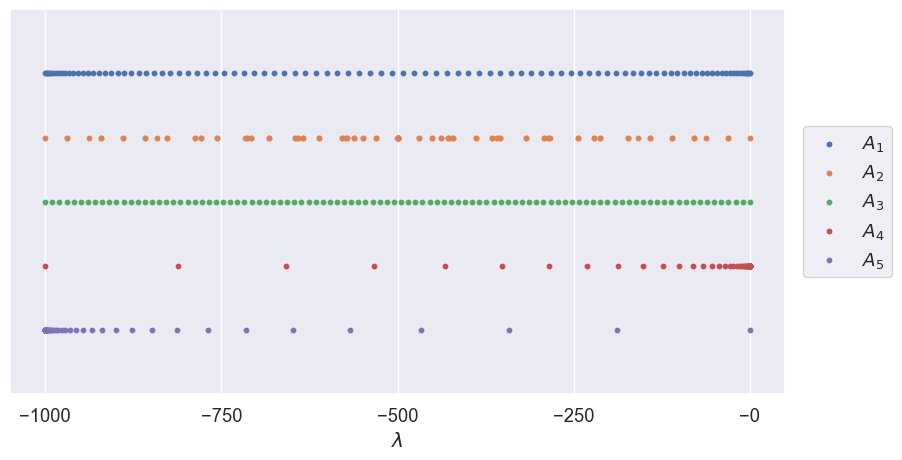
\includegraphics[width=.8\textwidth]{img/eigvals.png}
    \caption{
        Distribution of the eigenvalues of the test matrices with $n=100$ and
        $\lambda = 1000$.
    }
    \label{fig:eigenvaluedistributions}
\end{figure}

We are interested in computing $\varphi_p(tA) \mathbf{v}$ with $t \in \mathbb{R}$ being a time step.
We take $\hat{A}_{1D} \in \mathbb{R}^{n \times n}$ and $\hat{A}_{2D} \in \mathbb{R}^{n \times n}$
($n$ must have an integer square root), and we spectrally scale them so that they both have the
same spectral interval $[-\lambda, -\epsilon]$ with a parameter $\lambda > 0$ and $\epsilon = 0$.
We denote the resulting matrices by $A_1$ and $A_2$, respectively.
The spectral interval of a complex Hermitian or a real symmetric matrix is the smallest
interval in $\mathbb{R}$ that contains all the eigenvalues of the matrix, and it coincides
with the numerical range of the matrix.
Assuming that the spectral interval of the original matrix is $[\lambda_1, \lambda_n] \subset \mathbb{R^{-}}$,
the spectral scaling is done by $A_i = a \hat{A}_{iD} + b I$ for $i = 1, 2$; where the coefficients
are $a = (\lambda - \epsilon) / (\lambda_n - \lambda_1)$ and
$b = (- \lambda \lambda_n + \epsilon \lambda_1) / (\lambda_n - \lambda_1)$.
By scaling the matrices this way, we can focus on studying the effect of different eigenvalue
distributions on the same interval. The value of $\varphi_p(A_i) \mathbf{v}$ can then be
associated to $\varphi_p(t\hat{A}_{iD}) \mathbf{v}$ with $t \simeq \lambda / |\lambda_n|$ assuming that $\epsilon$
is sufficiently small and $\lim_{n \to \infty}\lambda_n = 0$,
which happens to be the case for $\hat{A}_{1D}$ and $\hat{A}_{2D}$. For $\hat{A}_{1D}$ with
$n = 10^4$, for instance, picking $\lambda = 10^5$ corresponds to $t \simeq 2.5\mathrm{e}{-04}$.


Beside these two matrices, we consider three diagonal matrices of size
$n \times n$, $A_3$, $A_4$, and $A_5$, with eigenvalues distributed on the same
interval, $[-\lambda, -\epsilon]$. The eigenvalues of $A_3$ are distributed
uniformly. The eigenvalues of $A_4$ and $A_5$ are distributed geometrically so that
they are concentrated on the right and the left ends, respectively. We test with
matrices with different $\lambda$'s and different sizes.
\autoref{fig:eigenvaluedistributions} shows the eigenvalues of these matrices with
$n=100$ and $\lambda = 1000$.

\subsubsection*{Pole Selection for Rational Krylov Subspace}

We use the \texttt{baryrat} library introduced in \cite{hofreither2021BRASIL} which implements
the AAA algorithm for rational approximations. One downside of using this algorithm
is the additional computational cost that it brings for computing the poles.
The AAA algorithm  computes the residual of the approximation on all the given interpolation points at
each iteration. Hence, for approximating a rational function of degree $m$, its computation cost scales
as $O(mq)$ where $q$ is the number of interpolation points given as input.
Furthermore, since this algorithm computes the poles based on the interpolation points, the
selected poles by this algorithm are very sensitive to the discretization of the interpolation domain.
Considering the $[-\lambda, 0] \subset \mathbb{R}$ interval, the number of interpolation
points for the AAA algorithm to work accurately scales with $\lambda$, which becomes a real burden
when $\lambda \to \infty$. However, as depicted in \autoref{fig:polesAAA}, numerical results show that
for this interval, the computed poles converge quite early when $\lambda$ is increased. We take
advantage of this behaviour and pre-compute the poles by running the AAA algorithm
on the interval $[-10^{4}, -10^{-16}]$ with $30000$ logarithmically spaced interpolation points.
The poles for $\varphi_1$, $\varphi_3$, $\varphi_5$, and $\varphi_{10}$ are pre-computed and stored.
Spacing the interpolation points logarithmically results in more interpolation points close to
the right end of the interval. This is better than spacing them uniformly because for the
exponential and the $\varphi$-functions, the gradients become very small as we go further away
from the origin to the left side of the real axis (i.e.,
as $\mathfrak{Re}(z) \to -\infty$ in \autoref{fig:scalarphifunctionscomplexplane}).

Using the poles from this strategy, the maximum errors of the scalar rational approximations on different
intervals have been computed and are presented in \autoref{fig:errorsAAAms}. These plots show that
it is possible to reach a maximum error of $10^{-12}$ with a degree less than $15$.
On the other hand, it has been observed that when the degree is increased, the computed poles
start taking values close to or on the negative real axis.
\autoref{fig:polesAAAms} illustrates this behavior for $\varphi_3$.
With $m=15$, we can see that some poles are getting close to the real negative axis. With $m=20$, 3 poles
lie on the negative real axis. With $m=25$, we can see that the situation is already very bad with many
poles lying on the negative real axis.
This can significantly impact the performance of the rational Krylov subspace approximation method if the input
matrix has real negative eigenvalues, which happens to be the case for our test matrices.
Comparing the computed poles with different number of interpolation points ($20000$ and $30000$)
in \autoref{fig:polesAAAms}, it can be concluded that when $m$ gets larger, more interpolation
points are needed in order to compute the poles accurately.
This justifies the unexpected increases in the errors in \autoref{fig:errorsAAAms}
for $\varphi_1$ and $\varphi_5$.

For a rational Krylov subspace of dimension $m$, we take $k \le m$ pre-computed poles $\eta_1, \dots, \eta_k$
by the AAA algorithm and we repeat them enough times to fill the $m$ poles $\xi_1, \dots, \xi_m$.
With this scheme for the pole selection, the rational Krylov subspace method is denoted by
\texttt{RA-AAAk} where \textit{k} is replaced by its value.
We also consider the case with a single repeated pole $\xi_1 = \xi_2 = \cdots = \xi_{m} = 1$ and
we deonte it by \texttt{RA-ONES}.

\begin{remark}
    In order to approximate the scalar function, the AAA algorithm needs to evaluate the scalar
    $\varphi_p(z)$ many times in the interval.
    For $\varphi_0$ the scalar exponential is used. For $\varphi_1$, the \texttt{scipy.special.expm1}
    function divided by $z$ gives accurate evaluations for large and small $z$.
    For $\varphi_p$, $p > 1$, two methods are used depending on the absolute value of $z$.
    For $|z| > 1$, \eqref{eq:scalarphifunctionsrecurrence} is used in a recursive algorithm.
    However, for small $|z|$, this method lacks numerical stability because of the numerical
    cancellation that happens in substracting the limit value
    $\lim_{z \to 0}\varphi_{p-1}(z) = \frac{1}{(p-1)!}$ from $\varphi_{p-1}(z)$.
    Hence, for non-zero $|z| < 1$, we use Corollary \ref{cor:embeddedmatrixexponential} and read $\varphi_p(z)$
    from the first entry of the last column of $\exp(\hat{A})$ with $\hat{A}$ being defined in
    \eqref{eq:embeddedmatrixdefinition} for the matrix-vector pair
    $(z \in \mathbb{C}^{1 \times 1}, 1 \in \mathbb{C}^{1})$.
\end{remark}

\begin{figure}[h!]
    \centering
    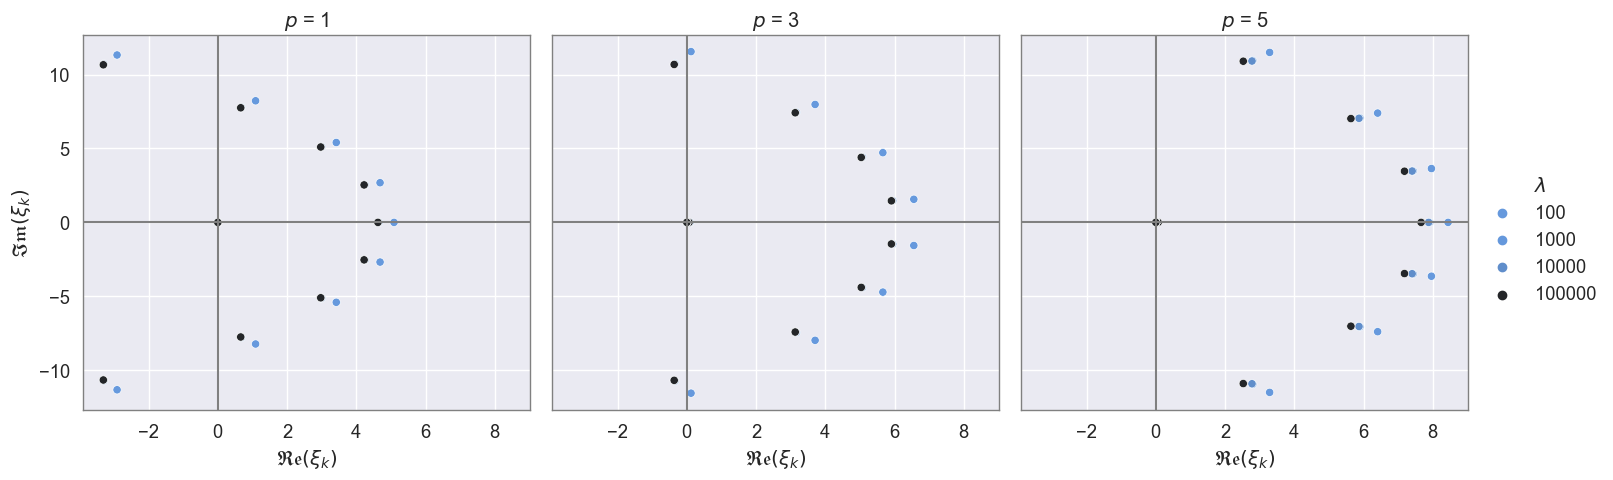
\includegraphics[width=.9\textwidth]{img/AAA/poles_lambda_log20k_m10.png}
    \caption{
        The first 10 poles computed by the AAA algorithm for $\varphi$-functions with $20000$
        logarithmically spaced interpolation points on the interval $[-\lambda, -10^{-16}]$.
    }
    \label{fig:polesAAA}
\end{figure}

\begin{figure}[h!]
    \centering
    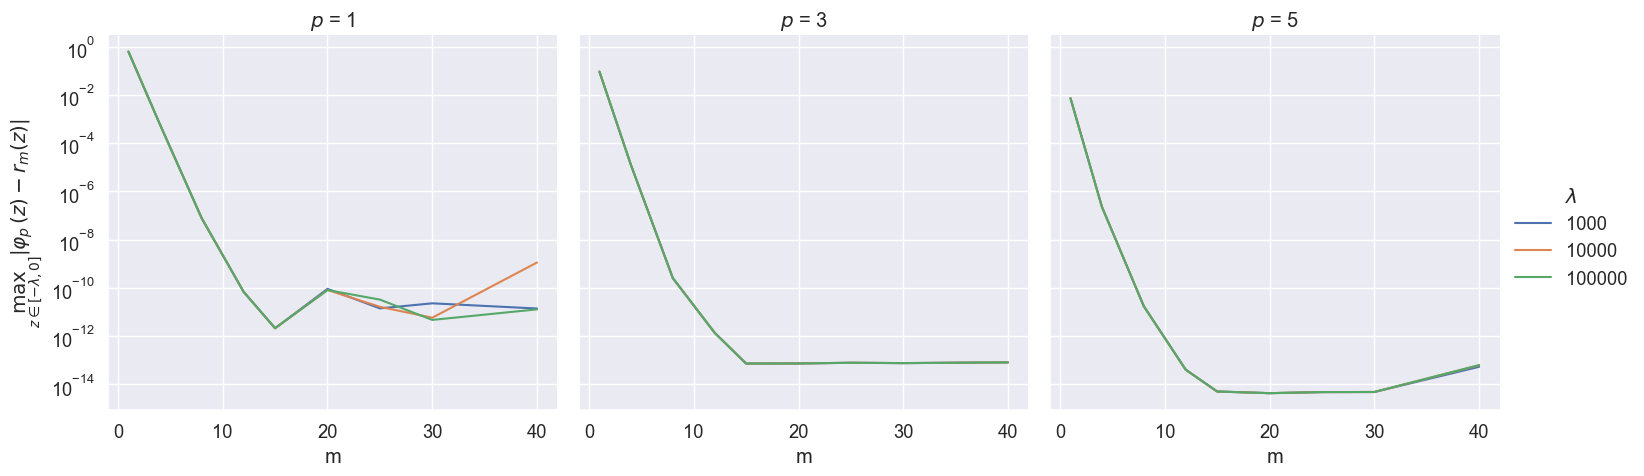
\includegraphics[width=.9\textwidth]{img/AAA/errors_ms_log30k.png}
    \caption{
        Maximum error of the rational approximation of scalar $\varphi$-functions
        on the interval $[-\lambda, 0]$.
        The approximations are done on the interval $[-10^4, -10^{-16}]$ with $30000$
        logarithmically spaced interpolation points.
    }
    \label{fig:errorsAAAms}
\end{figure}

\begin{figure}[h!]
    \centering
    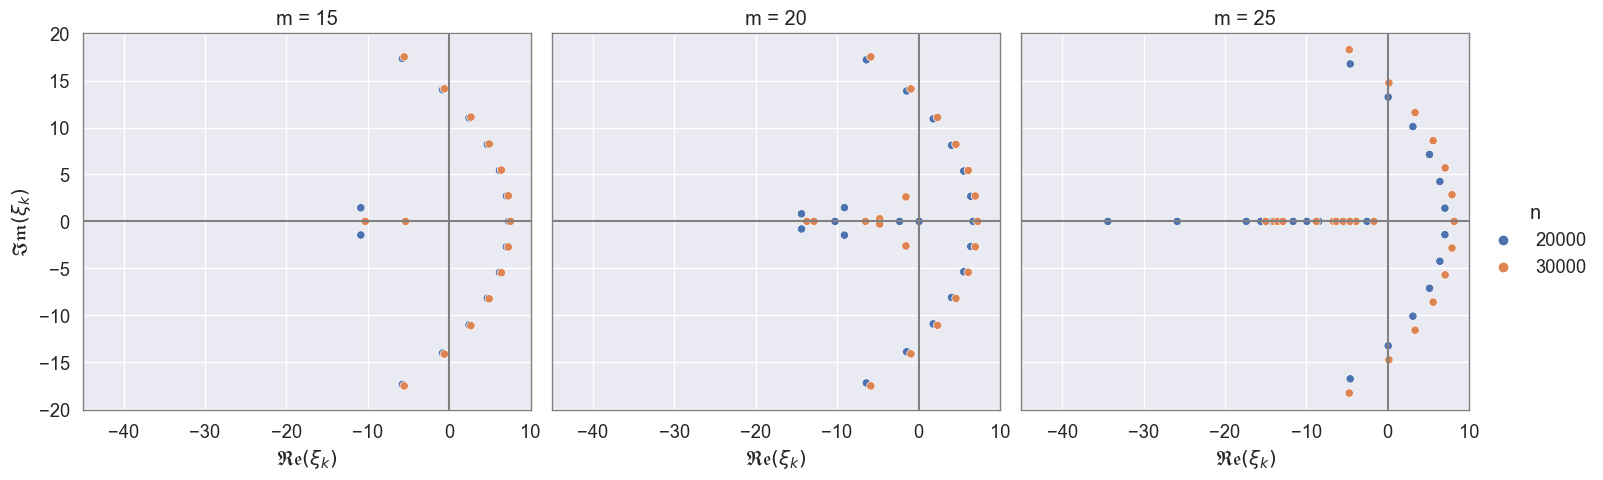
\includegraphics[width=.9\textwidth]{img/AAA/poles_ms_log_p03.png}
    \caption{
        Computed poles by the AAA algorithm for $\varphi_3$ with 20000 and 30000
        logarithmically spaced interpolation points on the interval $[-10^{4}, -10^{-16}]$.
    }
    \label{fig:polesAAAms}
\end{figure}

\FloatBarrier

\subsubsection*{Numerical Results}
The methods described in \autoref{sec:polynomialkrylovapproximation} (PA)
and \autoref{sec:rationalkrylovapproximation} (RA)
are implemented and their approximations have been evaluated for the test matrices.
For all the test matrices, the approximations are carried out for a normalized
random vector $\mathbf{v}$.
For computing $\exp(\hat{H}_m)$ and $\exp(\hat{A}_m)$, the \texttt{scipy.linalg.expm}
function from the the SciPy library~\cite{SciPy2020} is used which implements a
scaling and squaring algorithm with a Padé approximant for which the order is decided
based on the matrix~\cite{almohy2010scaling}.
In order to evaluate the approximation methods, we take the vectors computed by the methods
described in \autoref{sec:exactevaluation} as reference and we report the relative
error of the results from the Krylov subspace methods of dimension $m$, denoted by
$\mathbf{\Phi_{p, m}}$, against the reference vectors, denoted by $\mathbf{\Phi_p^{EX}}$.
The relative error is computed as:
\begin{equation*}
    \delta_{rel}(\mathbf{\Phi_{p, m}}) =
    \frac{\left\| \mathbf{\Phi_{p, m}} - \mathbf{\Phi_p^{EX}} \right\|_2}
    {\left\| \mathbf{\Phi_p^{EX}} \right\|_2}.
\end{equation*}

The convergence plots for the polynomial (top) and the rational (bottom) Krylov subspace approximations are
illustrated in \autoref{fig:krylovapproximationevaluation} for $A_1$ with size $n=10^{4}$.
Comparing the top and the bottom plots, it could be concluded that the RA method needs
much less iterations to converge.
Another major difference is the impact of the parameter $\lambda$ (the smallest eigenvalue).
With the polynomial Krylov subspace method, increasing $\lambda$ drastically slows down the convergence rate;
whereas the rational Krylov subspace method converges more or less with the same rate for
$\lambda=10^{3}$ and $\lambda=10^{5}$.
Furthermore, it can be observed that both methods always converge slightly faster for
larger $p$'s. This observation is consistent with the error bound provided in Lemma
\ref{lem:univariateerrorestimationphitaylor}, where we can see that increasing $p$ slightly
improves the bound. This slight improvement can also be justified by looking at the
$\varphi$-functions on the complex plane. As depicted in
\autoref{fig:scalarphifunctionscomplexplane}, when $p$ is increased, the
function $\varphi_p$ grows more slowly on the real axis and thus, its changes can be
captured better by a polynomial of a certain degree.
Therefore, the polynomial Krylov subspace approximation needs less iterations to reach a certain
tolerance according to Theorem \ref{the:univariateerrorestimationgeneral}.

\begin{figure}[h]
    \centering
    \begin{subfigure}[b]{.9\textwidth}
        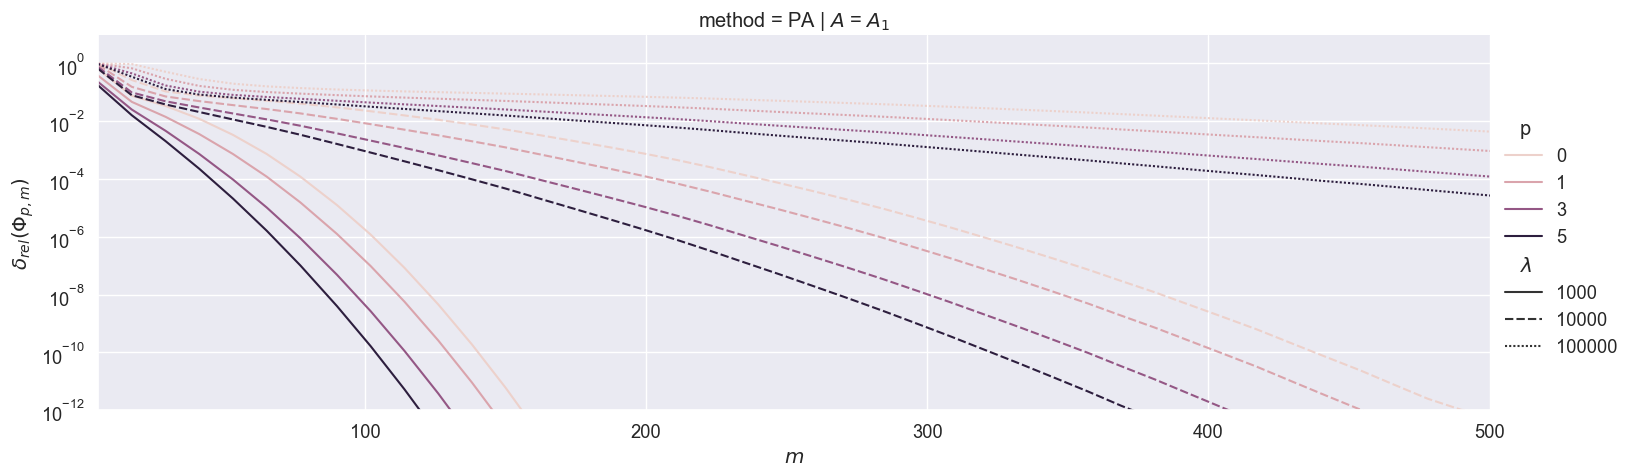
\includegraphics[width=\textwidth]{img/krylovapproximation/cnvg_ps_PA_n1e04.png}
        \caption{Polynomial Krylov subspace approximation.}
        \label{fig:polynomialkrylovapproximationevaluation}
    \end{subfigure}
    \vfill
    \begin{subfigure}[b]{.9\textwidth}
        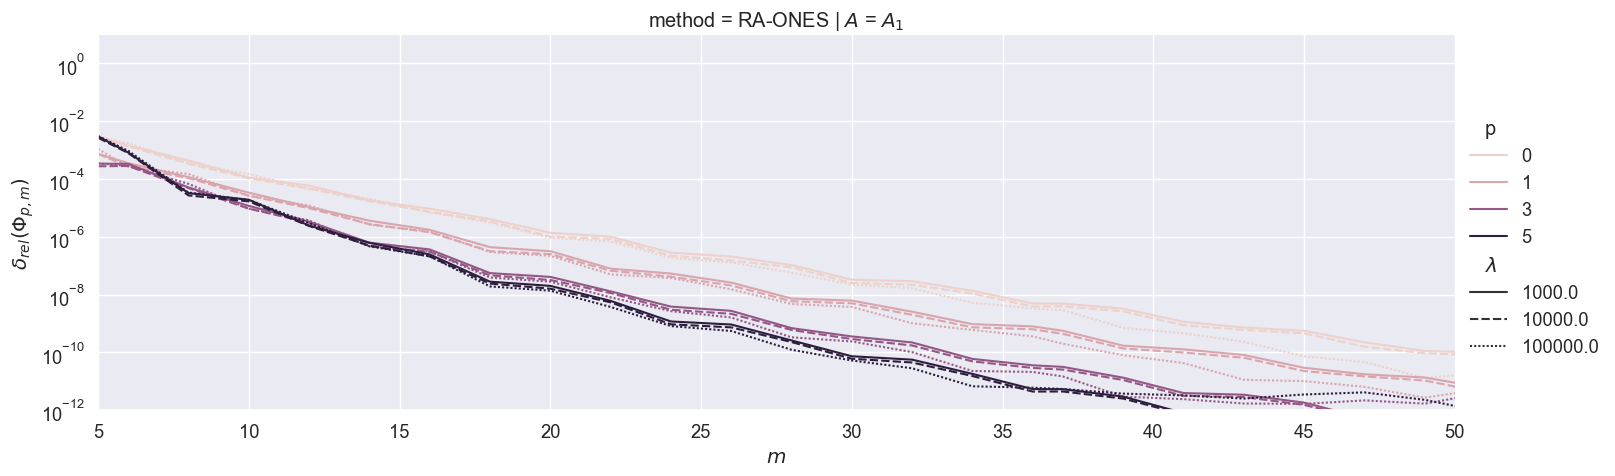
\includegraphics[width=\textwidth]{img/krylovapproximation/cnvg_ps_RA-ONES_n1e04.png}
        \caption{Rational Krylov subspace approximation.}
        \label{fig:rationalkrylovapproximationevaluation}
    \end{subfigure}
    \caption{
        Convergence of the approximations \eqref{eq:polynomialkrylovapproximation}
        and \eqref{eq:rationalkrylovapproximation} for matrices of size $n=10^{4}$.
    }
    \label{fig:krylovapproximationevaluation}
\end{figure}

\autoref{fig:krylovapproximationmatrices} compares the convergence of the test matrices
with the same numerical range (same $\lambda$).
With $\lambda = 10^3$, the method converges with almost the same rate for all the test matrices,
which is very close the rate estimated in \eqref{eq:univariateerrorestimationphi1}.
As $\lambda$ gets larger, we observe that the convergence for the matrices $A_2$ and $A_5$
gets considerably faster than for the other matrices.
What these two matrices have in common is that the distributions of their eigenvalues
(see \autoref{fig:eigenvaluedistributions}) are less dense on the right end of the
interval $[-\lambda, 0]$, where the scalar function has high gradients.
Therefore, for most of their eigenvalues, the polynomial approximant has a smaller error
compared to the other matrices.

\begin{figure}[h]
    \centering
    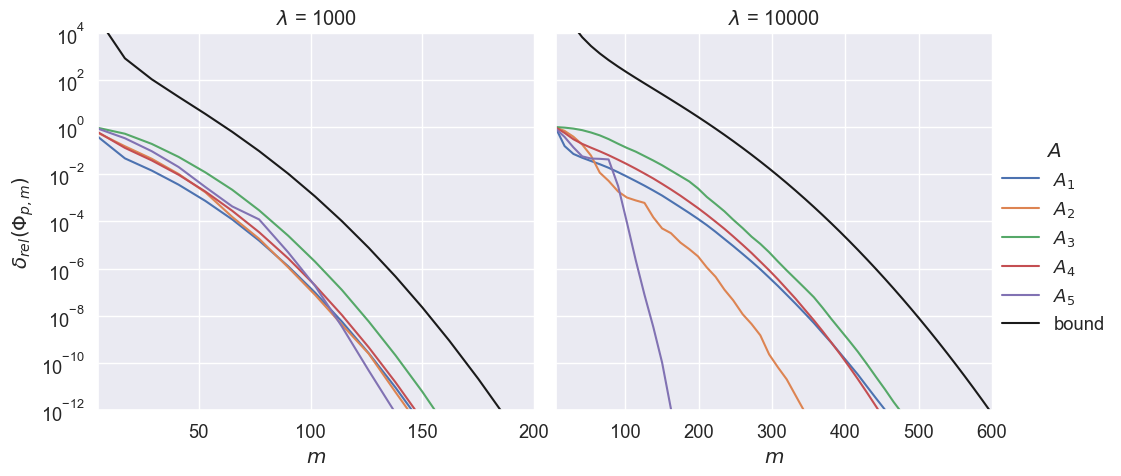
\includegraphics[width=.9\textwidth]{img/krylovapproximation/cnvg_matrices_PA_n10000.png}
    \caption{Convergence of the approximation \eqref{eq:polynomialkrylovapproximation}
    for $\varphi_1$ with different test matrices of size $n=10^4$ and the same spectral interval.
    The error estimation in \eqref{eq:univariateerrorestimationphi1} is plotted in black.}
    \label{fig:krylovapproximationmatrices}
\end{figure}

\autoref{fig:rationalkrylovpoleselection} compares the convergence of the
rational Krylov subspace method with different number of poles for $\lambda=10^3$ (top)
and $\lambda=10^5$ (bottom).
As expected, the method converges in less iterations when it is provided with more poles.
However, there is no improvement after $15$ poles as we can see that the plots of \texttt{RA-AAA30}
and \texttt{RA-AAA15} overlap. This observation is consistent with what has been observed
in \autoref{fig:errorsAAAms} for the scalar approximation errors.
From the scalar approximation errors, we also know that rational functions of degrees below
$10$ cannot approximate the $\varphi$-functions well enough. This is a compelling reason
for the failure of the methods \texttt{RA-AAA3}, \texttt{RA-AAA5}, and \texttt{RA-AAA7}.
With these methods, the relative error of the RA method stagnates after reaching a certain
value. However, this is not the case with only one or two repeated poles. The reasononing behind
this behaviour needs more consideration but it can originate from the fact that the poles
in \texttt{RA-AAA1} and \texttt{RA-AAA2} are real-valued.
Another interesting observation is that for \texttt{RA-AAA7} and \texttt{RA-AAA10}, the convergence
is very mcuh faster in the first "turn" of the poles (before they get repeated). It looks like
in the second turn and afterwards, the poles do not add as mcuh information to the subspace
as they do in the first turn; and therefore, we see a major drop in the convergence rate.
\texttt{RA-AAA15} and \texttt{RA-AAA30} converge before reaching the second turn, so this
behaviour cannot be seen for these approximations.

\begin{figure}[h]
    \centering
    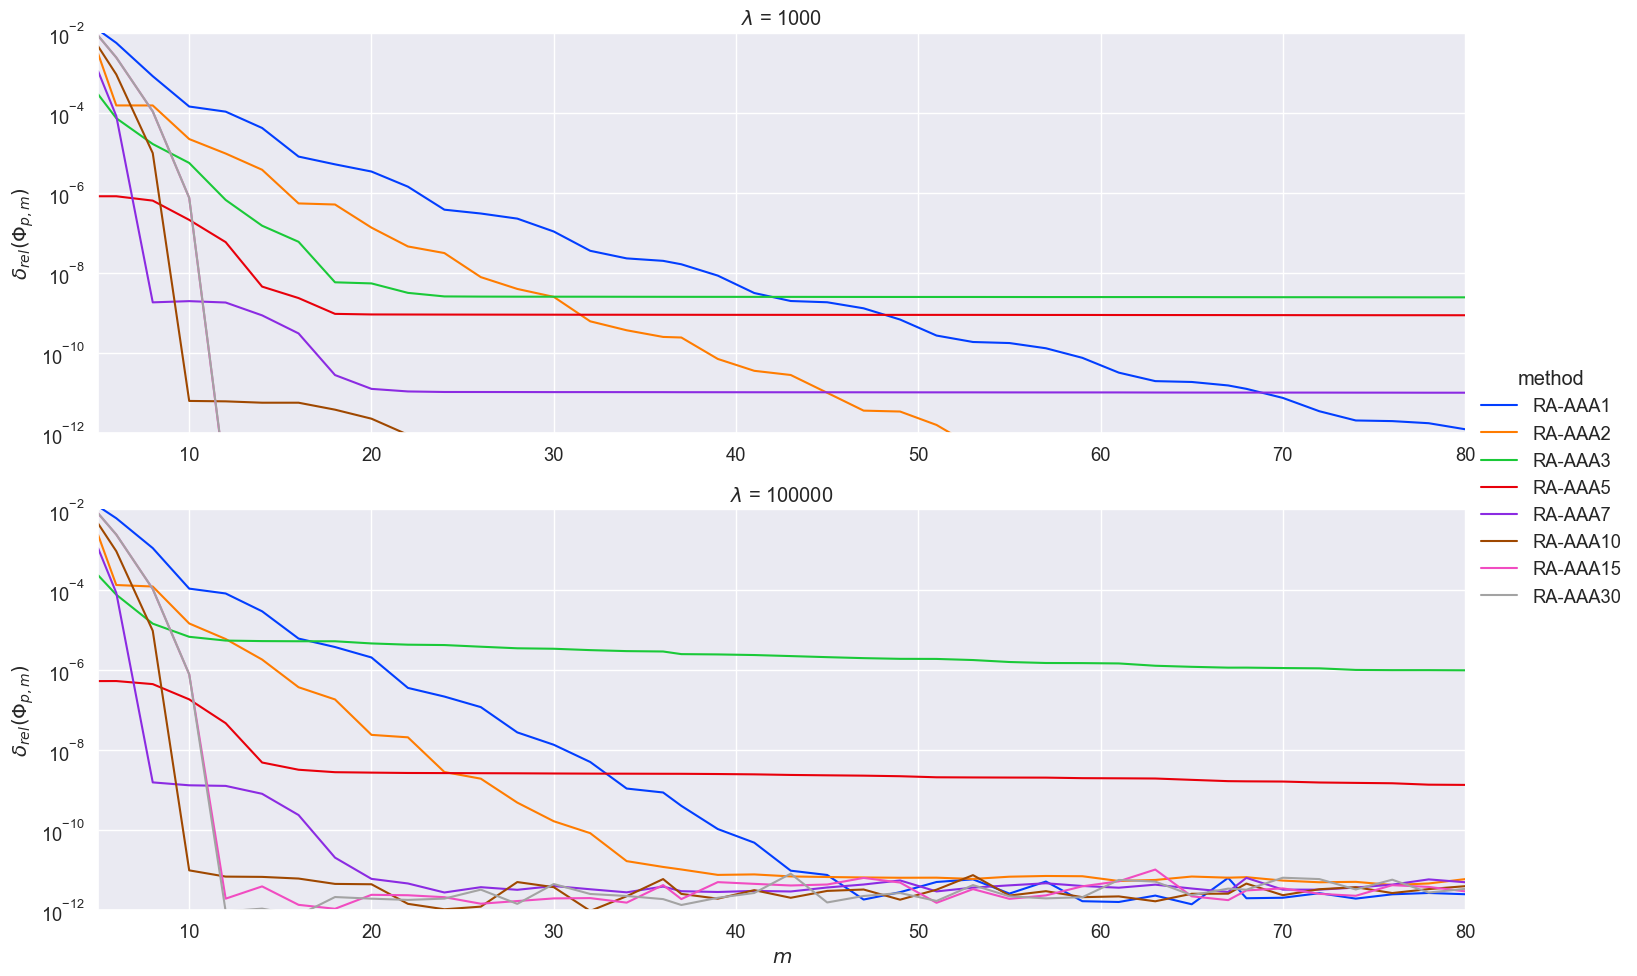
\includegraphics[width=.9\textwidth]{img/krylovapproximation/cnvg_poles_n1e04_p03.png}
    \caption{
        Convergence of the approximation \eqref{eq:rationalkrylovapproximation}
        for $\varphi_3(A_1^{n \times n})\mathbf{v}$ with different number of repeated poles for and $n=10^4$.
    }
    \label{fig:rationalkrylovpoleselection}
\end{figure}

So far, we have seen that using rational Krylov subspaces not only improves the convergence rate,
but it allows for larger $\lambda$'s as well which could be translated to larger time steps in
the context of exponential integrators.
However, these advantages come at a cost. In Algorithm \ref{alg:rationalarnoldi}, we need to
solve a linear system $m$ times. In the case of repeated poles, the algorithm benefits from pre-computing
the LU factorization of the corresponding matrices but it still needs to do the factorization
once for each pole. Therefore, for some cases, it might be more efficient to do more iterations
of the polynomial Krylov subspace method.
To address this issue, the process time of each method is presented in
\autoref{fig:krylovapproximationcputime} for the matrices $A_1$ (top row) and $A_2$
(bottom row) with different smallest eigenvalues and different sizes $n$.
The reported process time for each method corresponds to the minimum number of
iterations ($m$, dimension of the Krylov subspace) required by the method to reach
a relative error of $10^{-12}$ or smaller.
First of all, we can see that the computation time of the reference method (exponential of the
embedded matrix), denoted by \texttt{EX}, increases when the matrix becomes larger and when
its spectral interval becomes wider. Since the reference method implements an scaling and squaring
algorithm, it takes longer when the input matrix has a larger norm (larger $\lambda$).
With the polynomial Krylov subspace method, denoted by \texttt{PA}, although the performance
is acceptable for some cases, when the input matrix becomes larger, it becomes even slower than
the reference method especially with wider spectrums. Note that in the right top plot,
this method is not present because it does not converge even with 1000 iterations.
With the rational Krylov subspace method (denoted by \texttt{RA}), on the contrary,
the approximations can be computed very fast even for large matrices with wide spectrums.
However, we can see that when more poles are provided, the method becomes slower even
with less iterations. The \texttt{RA-AAA1} method is always the fastest one despite
needing more iterations to converge.
It should be noted that since the poles are pre-computed, the computation time of
the poles by the AAA algorithm is not included in the reported process times.

\begin{figure}[h]
    \centering
    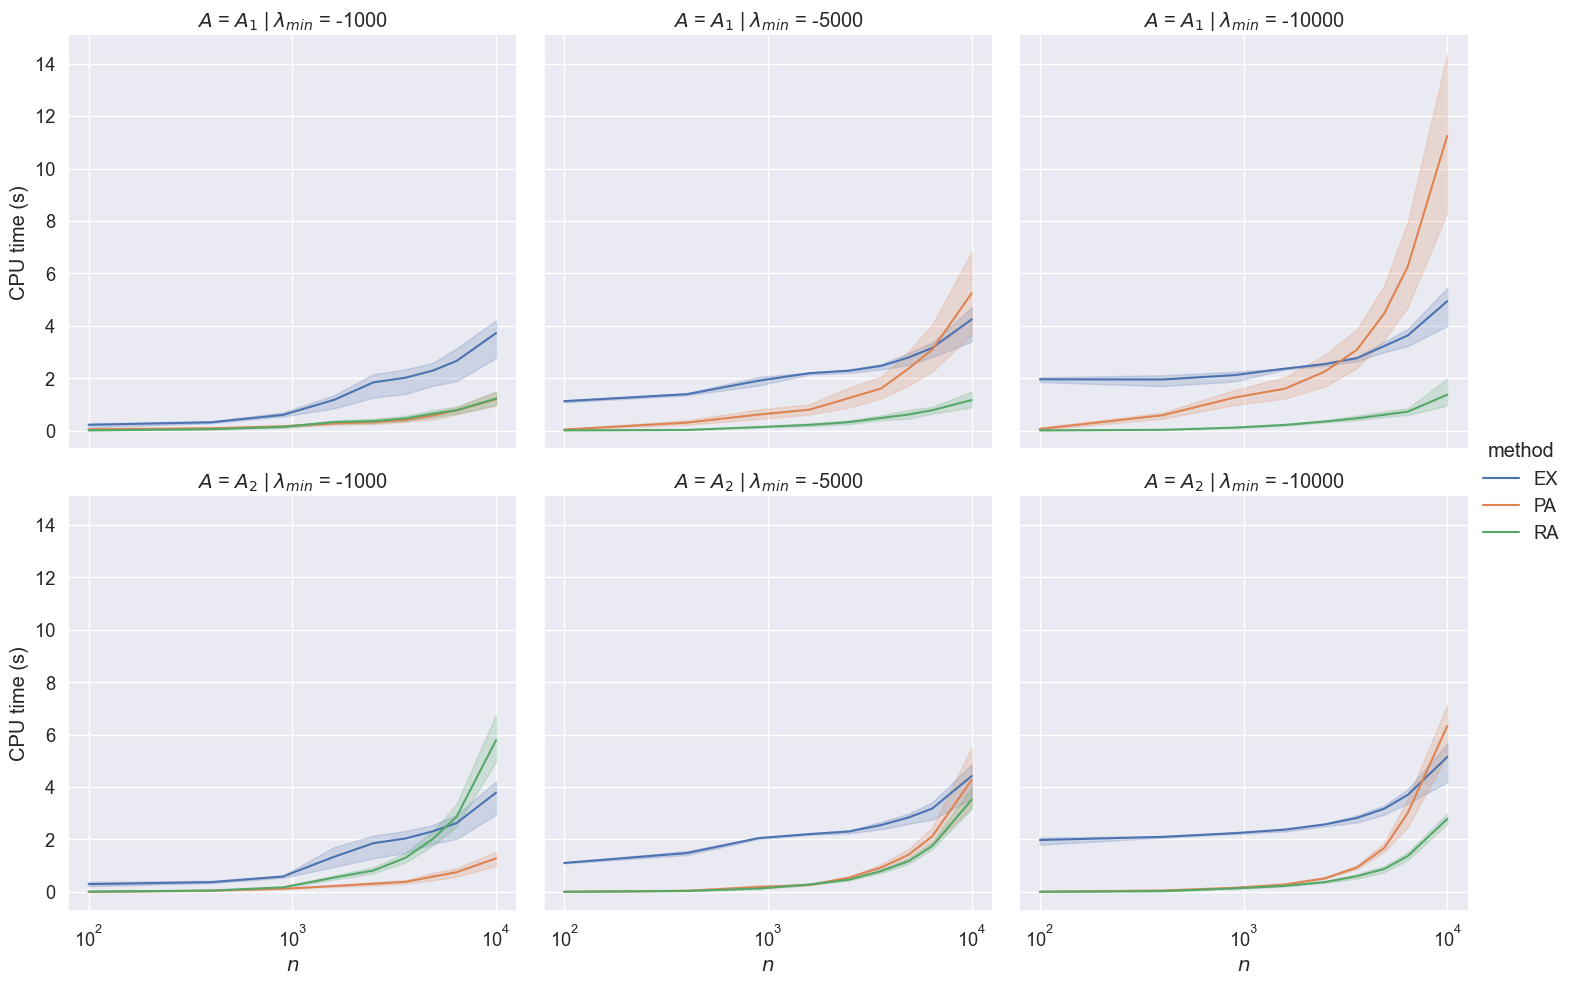
\includegraphics[width=.9\textwidth]{img/krylovapproximation/cputime_methods.png}
    \caption{
        CPU time for different evaluation methods. For the approximating methods,
        the minimum iterations required to reach a relative error less than $10^{-12}$
        is considered. Shadows of each line represent the range of the CPU time for
        $\varphi_0$, $\varphi_1$, $\varphi_3$, and $\varphi_5$.
        \texttt{EX} represents the reference evaluation.
    }
    \label{fig:krylovapproximationcputime}
\end{figure}

\FloatBarrier

\subsection{Trigonometric Functions}
\label{sec:resultstrigonometricfunctions}

Using finite elements for solving the PDE corresponding to a 2D linear elasticity problem,
\cite{voet2020linearelasticity} derives the following initial value problem
\begin{equation*}
    M \mathbf{\ddot{x}}(t) + K \mathbf{x}(t) = \mathbf{f}(t), \quad
    \mathbf{x}(0) = \mathbf{u'_0}, \; \mathbf{\dot{x}}(0) = \mathbf{v'_1},
\end{equation*}
where $M$ and $K$ are both symmetric positive definite matrices.
Computing the Cholesky factorization of $M = LL^{\top}$, pre-multiplying the problem by $L^{-1}$,
and a change of variables results
\begin{equation}
    \mathbf{\ddot{u}}(t) + A \mathbf{u}(t) = \mathbf{g}(t), \quad
    \mathbf{u}(0) = \mathbf{u_0}, \; \mathbf{\dot{u}}(0) = \mathbf{v_0},
\end{equation}
where
\begin{equation*}
    \begin{aligned}
        & \mathbf{u}(t) = L^{\top} \mathbf{x}(t), \quad & A = L^{-1} K L^{-\top}, \quad & \mathbf{g}(t) = L^{-1} \mathbf{f}(t), & \\
        & \mathbf{u_0} = \mathbf{u'_0}, & \mathbf{v_0} = \mathbf{v'_0}. & &
    \end{aligned}
\end{equation*}
Approximating $\mathbf{g}(t) \simeq \mathbf{g}(0) = \mathbf{g_0}$, the solution to
the problem satisfies
\begin{equation}
    \label{eq:elasticitysolution}
    \mathbf{u}(t) = \cos(t\sqrt{A}) \mathbf{u_0}
    + t \mathrm{sinc}(t\sqrt{A}) \mathbf{v_0}
    + \frac{t^2}{2} \mathrm{sinc}^2(\frac{t}{2} \sqrt{A}) \mathbf{g_0}.
\end{equation}

In this subsection, we investigate the performance of the presented methods in \autoref{sec:methods}
for approximating the three terms in \eqref{eq:elasticitysolution} with suitable time steps.

\subsubsection*{Test Matrices}
Since we are studying specific matrix functions for an specific problem, we will stick to the
matrices that appear for this problem. The matrix $A$ in \eqref{eq:elasticitysolution} is
calculated with the methods described in \cite{voet2020linearelasticity}:
$A_{LE}^{0.04} \in \mathbb{R}^{888\times888}$.

Unlike the test matrices in the previous subsection, this matrix is dense because
it is obtained by multiplying an sparse matrix by $L^{-1}$ and $L^{-\top}$ from left and
right. Nonetheless, it inherits the symmetry and the positive definiteness of $K$.
The square root of this matrix (computed by \texttt{scipy.linalg.sqrtm}) is also symmetric
positive definite, and its numerical range is:
\begin{gather*}
    % \mathcal{W}\left(\sqrt{A_{LE}^{0.10}}\right) = [9.96 \times 10^{5}, 2.59 \times 10^{6}],\\
    % \mathcal{W}\left(\sqrt{A_{LE}^{0.07}}\right) = [1.37 \times 10^{6}, 3.60 \times 10^{6}],\\
    \mathcal{W}\left(\sqrt{A_{LE}^{0.04}}\right) = [2.37 \times 10^{6}, 6.01 \times 10^{6}].
\end{gather*}

\subsubsection*{Pole Selection for Rational Krylov Subspace Approximation}
The pole selection strategy is the same as for $\varphi$-functions in \autoref{sec:resultsphifunctions},
using the AAA algorithm and repeating the poles.
The only difference is that the interpolation points are 2000 uniformly spaced points in the
numerical range of the input matrix. The arguments that justified the choice of logarithmic
distribution of the interpolation points are no longer true for the trigonometric functions.

\begin{figure}[h]
    \centering
    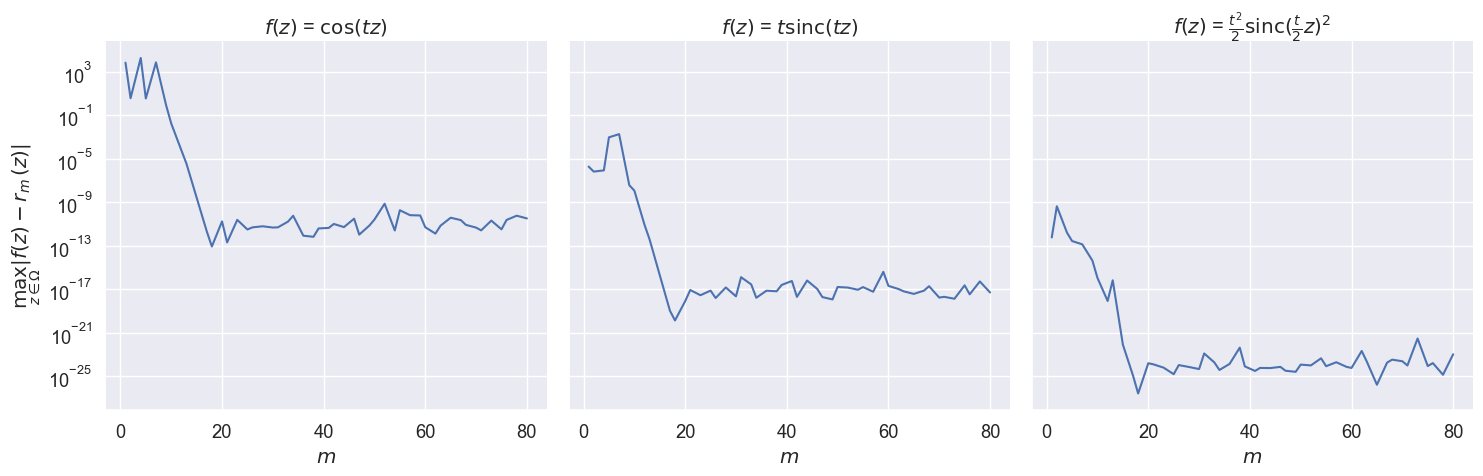
\includegraphics[width=.9\textwidth]{img/trigonometric/AAA_errors_t5e-06.png}
    \caption{
        Maximum error of the rational approximation of the trigonometric functions
        with $t=5\times10^{-6}$ on the interval $\Omega = [1 \times 10^{6}, 6 \times 10^{6}]$.
        The approximations are done by the AAA algorithm with $2000$ uniformly spaced
        interpolation points.
    }
    \label{fig:trigonometricAAAerrors}
\end{figure}

The absolute errors of the rational approximations of the scalar functions are presented in
\autoref{fig:trigonometricAAAerrors}.
For all three functions, the errors do not decrease when the degree of the rational function is too low.
This behaviour lies on the oscillatory nature of the trigonometric functions. When the degree is increased,
at some point, the rational functions become powerful enough to capture the oscillations and the errors
start decreasing. With a degree around $20$, the functions reach their full potential and there is no
improvement afterwards. This \textit{minimum sufficient} degree is higher for bigger time steps.
For $t = 2 \times 10^{-5}$, for instance, a rational function of degree at least $40$ is needed.
Note reason that the starting absolute errors are very small is that the values of the functions
$f(z)=t \mathrm{sinc}(tz)$ and $f(z)=\frac{t^2}{2} \mathrm{sinc}(\frac{t}{2}z)^2$ are small because
of their leading coefficients.

\FloatBarrier

\subsubsection*{Numerical Results}

The methods described in \autoref{sec:polynomialkrylovapproximation} (PA)
and \autoref{sec:rationalkrylovapproximation} (RA) have been evaluated for the presented test matrices.
For all the test matrices, the approximations are carried out for a normalized random vector $v$.
For computing the cosine and the sine of the matrices $\hat{H}_m$ and $\hat{A}_m$ in the PA and the
RA methods, respectively, the \texttt{scipy.linalg.cosm} and \texttt{scipy.linalg.sinm} function
from the the SciPy library~\cite{SciPy2020} are used which use the \texttt{scipy.linalg.expm}
function internally.
Similar to \autoref{sec:resultsphifunctions}, we take the vectors computed by the methods
described in \autoref{sec:exactevaluation} as reference and we report the relative
error of the results from the Krylov subspace methods of dimension $m$, denoted by
$\mathbf{f_m}$, against the reference vectors, denoted by $\mathbf{f^{EX}}$.
The relative error is computed as:
\begin{equation*}
    \delta_{rel}(\mathbf{f_m}) =
    \frac{\left\| \mathbf{f_m} - \mathbf{f^{EX}} \right\|_2}
    {\left\| \mathbf{f^{EX}} \right\|_2}.
\end{equation*}

The relative errors of the approximations with different dimensions of Krylov subspaces
are presented in \autoref{fig:trigonometricconvergences} with the time steps
$t=5 \times 10^{-6}$ (top) and $t=2 \times 10^{-5}$ (bottom).
With the polynomial Krylov subspace approximation (PA), the error does not decrease when
the dimension of the Krylov subspace is too low. This is similar to what has been
observed in \autoref{fig:trigonometricAAAerrors} and it is again because of the
oscillations of trigonometric functions.
With the rational Krylov subspace approximations (RA), the performance is not satisfactory in general.
The main reason is that when only a portion of the poles are provided (i.e., when $m < k$),
the rational functions are not able to approximate the functions well. We can see that
the relative error of the \texttt{RA-AAAk} method suddenly drops when the dimension of
the subspace reaches $k$ and all the poles have been used. For this reason, the convergence
of this method is delayed by the number of the poles. On the other hand, if $k$ is not large
enough, the rational functions are not powerful enough to approximate the scalar functions
(see \autoref{fig:trigonometricAAAerrors}).
This is evident in the bottom row of \autoref{fig:trigonometricconvergences} where the method
does not converge with $20$ poles and it can only reach an error of $10^{-8}$ with $30$ poles.

The observations in the bottom row of \autoref{fig:trigonometricconvergences} gives the
idea that there might be some potential advantages in the RA method for bigger time steps,
if the pole selection strategy is improved. In an attempt for improving the pole selection
strategy, we did the same experiments by using the poles from the AAA algorithm only once
and using $\xi_i = \infty$ for $i > k$. Since the rational Krylov subspace with infinity
poles is identical to the polynomial Krylov subspace, the idea here is to benefit from
the poles in the first $k$ iterations and do the same as in polynomial Krylov subspace
in the rest of the iterations. The resulting subspace will contain rational functions
of the type $(m, k)$ when $k \le m$.
\autoref{fig:trigonometricconvergences_mk} shows the relative errors for the time step
$t = 2 \times 10^{-5}$. Although there are some improvements for the dimensions $m > k$,
especially for \texttt{RA-AAA20}, this strategy did not solve the main problem of the
RA method. The convergence still loses momentum when the dimension of the subspace
reaches $k$.

\begin{figure}[h]
    \centering
    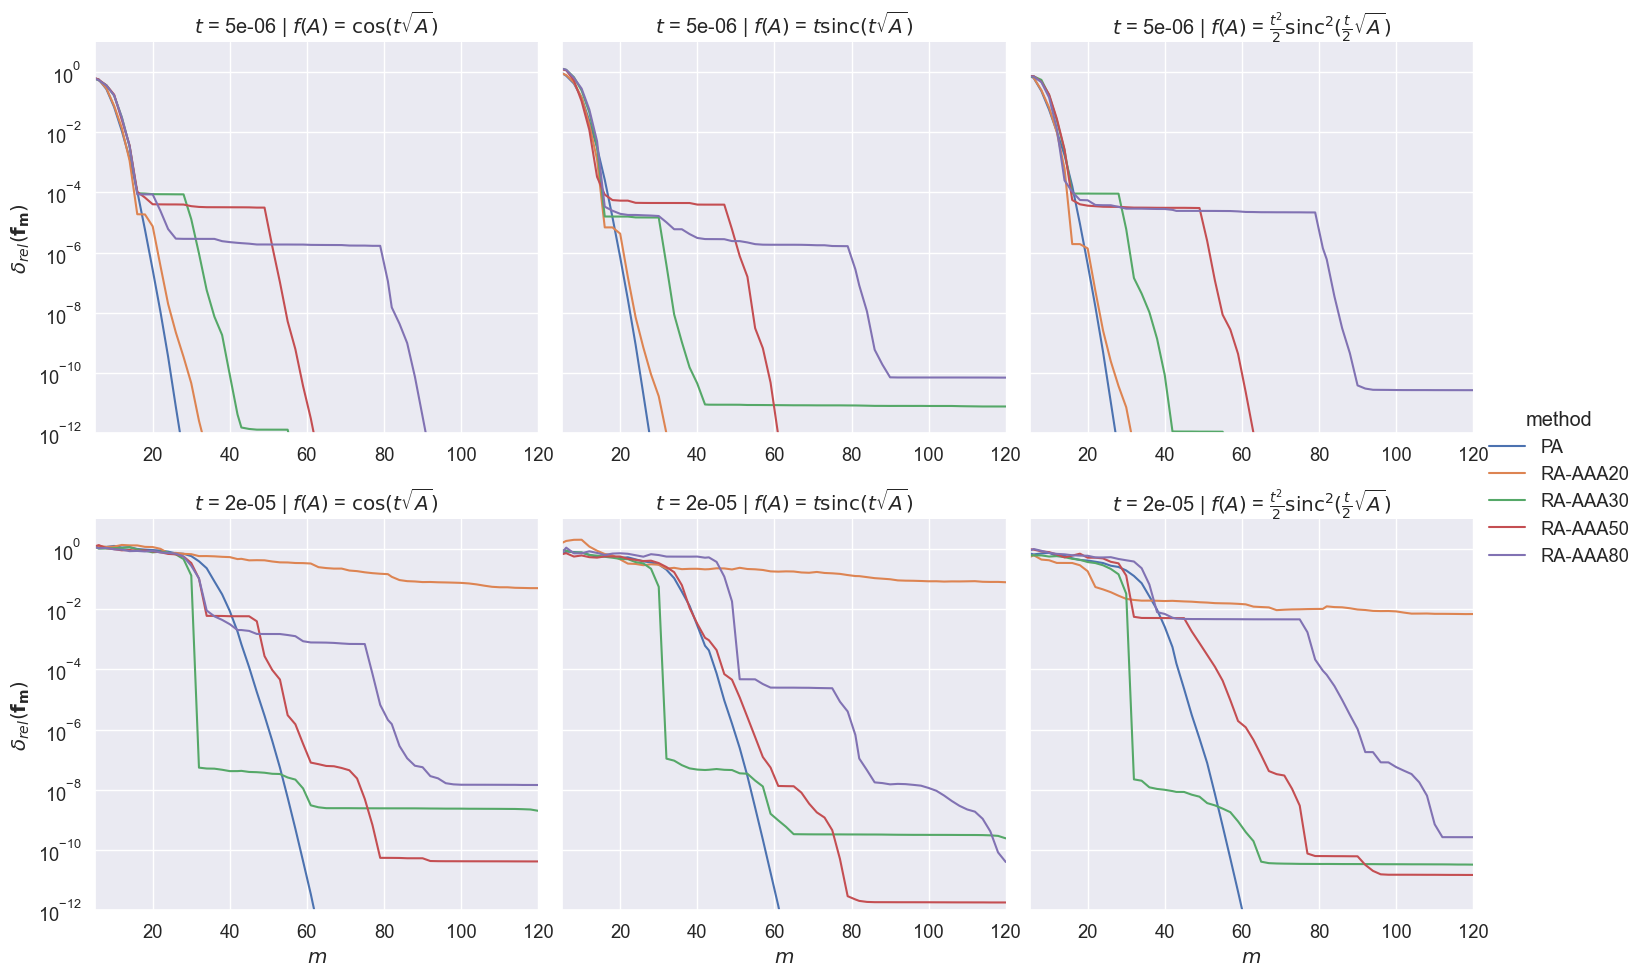
\includegraphics[width=.9\textwidth]{img/trigonometric/cnvg_h4e-02_methods_ts.png}
    \caption{
        Convergence of the approximations \eqref{eq:polynomialkrylovapproximation}
        and \eqref{eq:rationalkrylovapproximation} for $A_{LE}^{0.04}$. Each column
        shows plots for one function. Each row shows plots for one time step.
        }
        \label{fig:trigonometricconvergences}
\end{figure}

\begin{figure}[h]
    \centering
    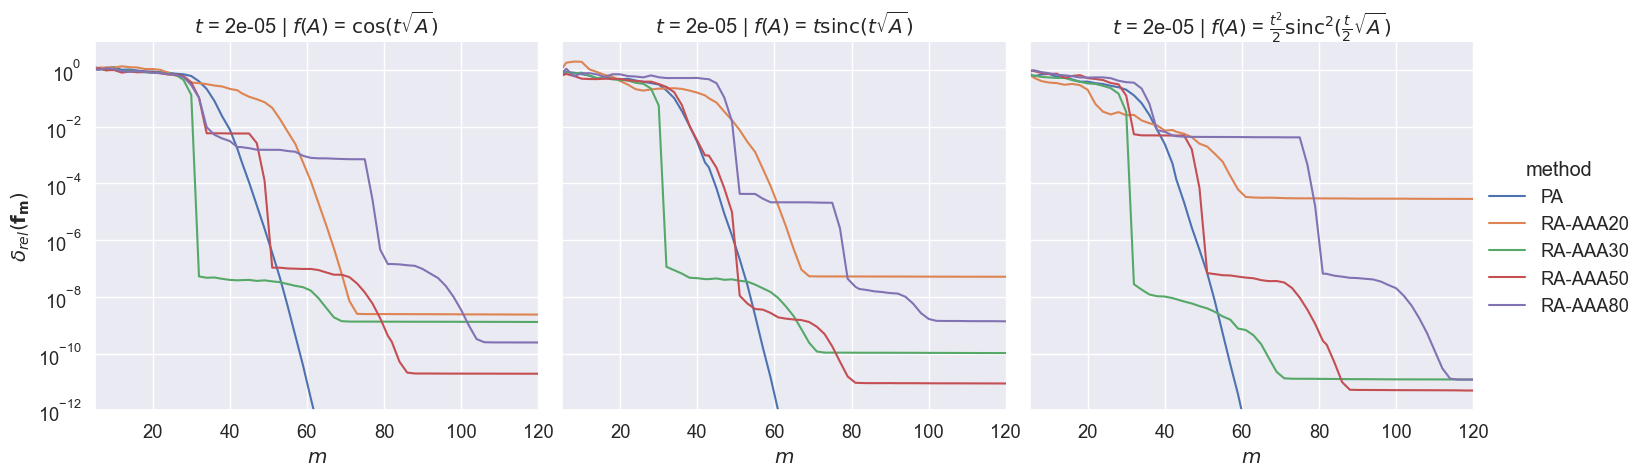
\includegraphics[width=.9\textwidth]{img/trigonometric/cnvg_h4e-02_methods_ts_mk.png}
    \caption{
        Convergence of the approximations \eqref{eq:polynomialkrylovapproximation}
        and \eqref{eq:rationalkrylovapproximation} with rational functions of type
        $(m, k)$ for $A_{LE}^{0.04}$.
        Each column shows plots for one function.
        }
        \label{fig:trigonometricconvergences_mk}
\end{figure}

\FloatBarrier

\section{Conclusion}
\label{sec:conclusion}

In this work, we investigated the performance of polynomial and rational Krylov subspace
methods for approximating the action of $\varphi$-functions and trigonometric matrix
functions on a given vector for real symmetric matrices.

For the $\varphi$-functions, we focused on the interval $(-\infty, 0]$ and parameterized
the spectrum of the input matrix as $[-\lambda, 0]$ with $\lambda > 0$. We studied the
convergence for different $\lambda$'s.
In the context of exponential integrators, the spectrum of the input matrix usually
depends on the the time step and other parameters (e.g., mesh size, underlying PDE)
that are out of hand.
Therefore, we can translate our findings about the effect of the parameter $\lambda$ to
the time step in exponential integrators.
Here is a summary of the main findings of this work for the $\varphi$-functions:
\begin{itemize}
    \item The approximation of higher order $\varphi$-functions with polynomials
        and rational functions is slightly easier because of they change more slowly
        on the left half complex plane (see \autoref{fig:scalarphifunctionscomplexplane}).
    \item The poles of the rational functions can be pre-computed on a sufficiently
        large interval and be used for all time steps.
    \item The rational Krylov subspace method needs less iterations to converge.
        Furtheremore, contrary to the polynomial Krylov subspace method, it allows for
        bigger time steps without increasing the number of the iterations
        (dimension of the Krylov subspace).
    \item The rational Krylov subspace method benefits from poles that are returned by
        the AAA algorithm.
        However, one needs to be careful to provide it with sufficient number of poles
        since it might not converge with only a few poles, unless they are all real-valued.
        The improvement of the method is a direct impact of the improvement of the scalar
        approximations.
    \item Regarding the computation time for large sparse matrices, the polynomial
        approximation performs even slower than the baseline methods
        (scaling and squaring methods for $e^A$) when the time step is increased.
        The rational Krylov subspace method with one or two repeated pole should always
        be the method of choice. Despite taking more iterations to converge, it returns
        in less time compared to using more poles, especially when the time step is bigger.
\end{itemize}

For the trigonometric functions, we focused on the 2D linear elasticity problem and
applied the methods on dense matrices.
Here is a summary of the main findings for the trigonometric functions:
\begin{itemize}
    \item Because of the oscillatory nature of the functions that have been studied,
        the approximation errors do not change much before a minimum dimension of
        Krylov subspace is reached.
    \item The polynomial Krylov subspace method needs more iterations to covnerge
        when the time step is increased.
    \item The convergence of the rational Krylov subspace method is delayed until
        the subspace has been fed with all the poles from the AAA algorithm.
        Also, when the dimension of the Krylov subspace surpasses the number of the
        the poles, repeating the poles or using infinity will not help for these functions.
\end{itemize}

For the rational approximations, we focused on the AAA algorithm for choosing the poles.
Since this algorithm is based on interpolating the scalar function on a set of given
points, it has the disadvantage that it does not allow for restricting the poles.
In the case of the $\varphi$-functions, restricting the poles to real positive values
or far from the negative real axis might be of interest.
We saw in \autoref{fig:rationalkrylovpoleselection} that the method converges even with
only a few repeated poles (\texttt{RA-AAA1} and \texttt{RA-AAA2}), provided that the poles
are real. However, it might not converge if some of the poles are complex.
It remains for a future work to investigate the theoretical reason behind this behaviour.
In the case of one real repeated pole, the method has been linked to the shift-and-invert
method (see Section 7.4 of \cite{guttel2010rational}).
